\documentclass[11pt, a4paper, notitlepage]{article}
\usepackage{graphicx}   
\usepackage{wrapfig}  
\usepackage{url}
\usepackage{float}
\usepackage{caption}
\usepackage{subcaption}
\usepackage[margin=3cm]{geometry}

\title{Mathematics into School - Project Report}
\author{Tom Mann}
\date{\today}

\begin{document}

\maketitle

\begin{abstract}
    %TC:ignore
    This report details a project delivered in partnership with Our Lady and st Thomas Catholic Primary School, aiming to increase girls' confidence in mathematics and reduce levels of maths anxiety. Over a series of six sessions, a group of Year 6 girls engaged with a variety of mathematical activities. The pedagogical insight behind the content, design and delivery of these sessions will be examined. Finally, the report will evaluate the success of the project with regard to building confidence, reducing anxiety, along with the legacy to the students.
    %TC:endignore
\end{abstract}

% TODO: Add a word count

\tableofcontents

\clearpage

\section{Introduction}

\subsection{Context}
This project was conducted in partnership with Our Lady and St Thomas School (OLST), a  co-educational Catholic primary school with approximately 120 students. The school demonstrates strong academic results; the percentage of students achieving expected or a higher standard in reading, writing and maths is above the national and local average \cite{OLST_stats}.
\par
However, it has been observed that some girls in the Year 6 class lack confidence in maths lessons and participate less actively than hoped. One study found that boys tend to initiate more exchanges whereas girls prefer to be respondent, to be called on by a teacher \cite{Rashid:2012}. While some of this contrast in preference may be explained by biological differences, it may be that there is a confounding variable such as self-confidence and anxiety. 


\subsection{Aims}
There were two main aims for the project, although they may appear similar and overlap in some aspects they are distinct.

\subsubsection*{Aim 1 -- Increasing self-confidence in girls in maths} 
Confidence within any subject is the belief that you can rely on your own abilities. From this definition it appears that there are two primary ways to increase self-confidence: either improve students' abilities, or strengthening their belief in their own abilities. Nationally and in the North East the percentage of girls and boys achieving the expected standard in their maths SATs has been within 2 percentage points of each other since 2018/19 \cite{maths_SATs_stats}. This suggests that while improving mathematical ability may increase girls confidence this may not be the main cause of a lack of self-confidence when compared with the boys in the class.
\par
One study  found two differences in the mindset of girls and boys in regard to taking responsibility for success and failure. Firstly ``girls tend to attribute failure in mathematics to a lack of ability, whereas boys attribute failure to a lack of effort", and secondly, girls are more likely to attribute success to external factors, such as an easy exam \cite{Georgiou01122007}. This creates a dichotomy in which many girls take responsibility for their failures but do not credit themselves for their successes. Consequently it was decided the best way to tackle self-confidence was in the mindset of girls.
\subsubsection*{Aim 2 -- Decreasing maths anxiety in girls}
Maths anxiety is broadly defined as a feeling of worry or nervousness, often accompanied by physiological reactivity, towards current or future situations involving maths \cite{Luttenberger:2018}. While this is related to low self-confidence, it is possible for students to experience one without the other. Similarly to self-confidence, girls appear to be disproportionately affected. The National Numeracy survey found that women were twice as likely to experience maths anxiety as men \cite{NationalNumeracy_anxiety}; however it is important to note general anxiety is also higher amongst girls.
\par
It has been found that there is a negative relationship between maths anxiety and maths performance, i.e. higher maths anxiety is linked to poorer mathematical achievement \cite{Chang:2016}. 
Although there are various studies around the cause-and-effect relationship between maths anxiety and maths performance, it is not widely agreed upon if one causes the other --- some researchers propose that the relationship may be cyclic \cite{Chang:2016}. 
\par
Therefore, treating maths anxiety solely by improving performance may be insufficient. When dealing with maths anxiety it is important to treat both the cause and the symptoms. Treating the symptoms of anxiety is more aligned with behavioural therapy,  whereas this report will focus on treating the cause of maths anxiety.

\subsection{Introduction to Students}
Due to the nature of the aims, this project is very individual. It was decided to spend some time learning about student's experiences before designing the sessions. One session was dedicated to speaking with the girls in the Year 6 class to better understand the prevalence and causes of maths anxiety amongst them.
\par
 All of the students agreed that they had felt worried during maths lessons at some point. As it became clear that maths anxiety was common across the group, it was deemed unnecessary to explore individual experiences in depth; instead the focus shifted to identifying common causes of anxiety. The girls identified three main factors contributing to their maths anxiety: fear of failure, fear of judgement, and fear of being left behind. One student added that maths can feel frustrating because, when they do not understand something, they feel stuck and unable to progress. It was with these insights in mind that the sessions were designed.

\section{Activities}

\subsection{Structure}
This project took place with a Year 6 class containing eight girls. It was decided to include all the girls from the class in each 30-minute lunchtime session. This may have reduced the amount of time that could be spent with each student; however, in such a small class excluding only a few students would be unfair and undermine the aim of boosting girls' confidence.
\par
The decision to include only girls in the group was made not just from a logistics perspective, it also brings pedagogical benefits. research has shown that boys and girls may perform better in different learning environments, these differences include the use of space, movement and collaboration \cite{Hughes:2006}. Including only girls means the sessions could be tailored to suit their learning styles best. As mentioned previously, girls tend to prefer to respond when called upon rather than volunteer answers. Including only girls provides the opportunity for the girls to get comfortable initiating more exchanges.
\par 
It has been found that maths anxiety is often linked to teaching style, in particular in a traditional classroom setting the teacher takes an authoritative role \cite{Finlayson:2014}. To address this, the sessions were delivered around a group table with everyone sitting to reduce my presence as a directive role. 


\subsection{Session 2: M\"obius strips}
This session was designed with two strategies for dealing with maths anxiety in mind. The first stems again from the link between delivery methods and maths anxiety, in particular traditional delivery methods focus on the outcome of a lesson, whether that be students gaining specific knowledge or being able to answer certain questions correctly. The remedy to this is a more constructivist approach to teaching, focusing on the process rather than the product \cite{Finlayson:2014}. The second strategy is based on Expectancy-Value Theory, ``ACER's Mathematics anxiety and Engagement Strategy" outlines four different types of value that are important for motivation; we shall focus on intrinsic value in this session and utility value later on \cite{MAES:2024} . Intrinsic value comes simply from finding value in maths because you find it interesting or enjoyable.
\par
To align with the goal of focusing on the process of learning, the first session was created with no learning outcome in mind, that is there are no expectations for the students to learn or recreate anything from the session. The intrinsic value of the session comes from exploring a shape the students will never have seen before, with properties they will never have seen before. 
\par
A M\"obius strip (see Figure 1) is created by taking a strip of paper, giving it a half-twist, and then joining the ends together. This creates a one-sided, one edged surface. The session consisted of the students working in pairs to: make, draw on and cut the M\"obius strips. These aspects of the session align with two constructivist methods, group work and manipulation of materials as a primary source of information. 
\par
There was a demonstration in front of the students of how to create a M\"obius strip, they then worked in pairs, sometimes with external help to construct their own M\"obius strip. The students were then told to draw lengthwise along the M\"obius strip until they get back to the start. This appears to end up with a line on ``both" sides of the shape even though the students only drew one line. Through this task alone the students didn't realise the surface only had one side, so they were asked a slightly incorrect question of ``You only drew on one side, but there is a line on both sides, how is this possible?". Through constructing and deconstructing more M\"obius loops the students explored how a surface can have only one face.
\par
The next task involved the students cutting down the line they had drawn. Unexpectedly the surface does not end up in two pieces, but stays as one loop with more twists in it. This property was impossible for the students to miss when they completed this task. This property was more difficult to explain simply by building M\"obius strips. The session was adapted and a prop was made by writing left and right at the ends of the strip. When the strip of paper was joined without a twist, the left and right lined up at the join as expected. The students could then observe that when we add a half-twist to make a M\"obius strip that left joins with right and vice versa (see Figure 2). This showed that when they cut the strips there is no left and right side for them to split into. Note, here left and right do not have any meaning and are only to show that the sides do not join as expected. 

\begin{figure}[htbp]
    \centering
    \begin{minipage}{.48\textwidth}
      \centering
      \includegraphics[height=.39\linewidth]{Images/Möbius_Strip.jpg}
      \captionof{figure}{Example of a M\"obius strip, the one-sided surface created by adding a half twist to a strip of paper }
      \label{fig:test1}
    \end{minipage}%
    \hfill
    \begin{minipage}{.48\textwidth}
      \centering
      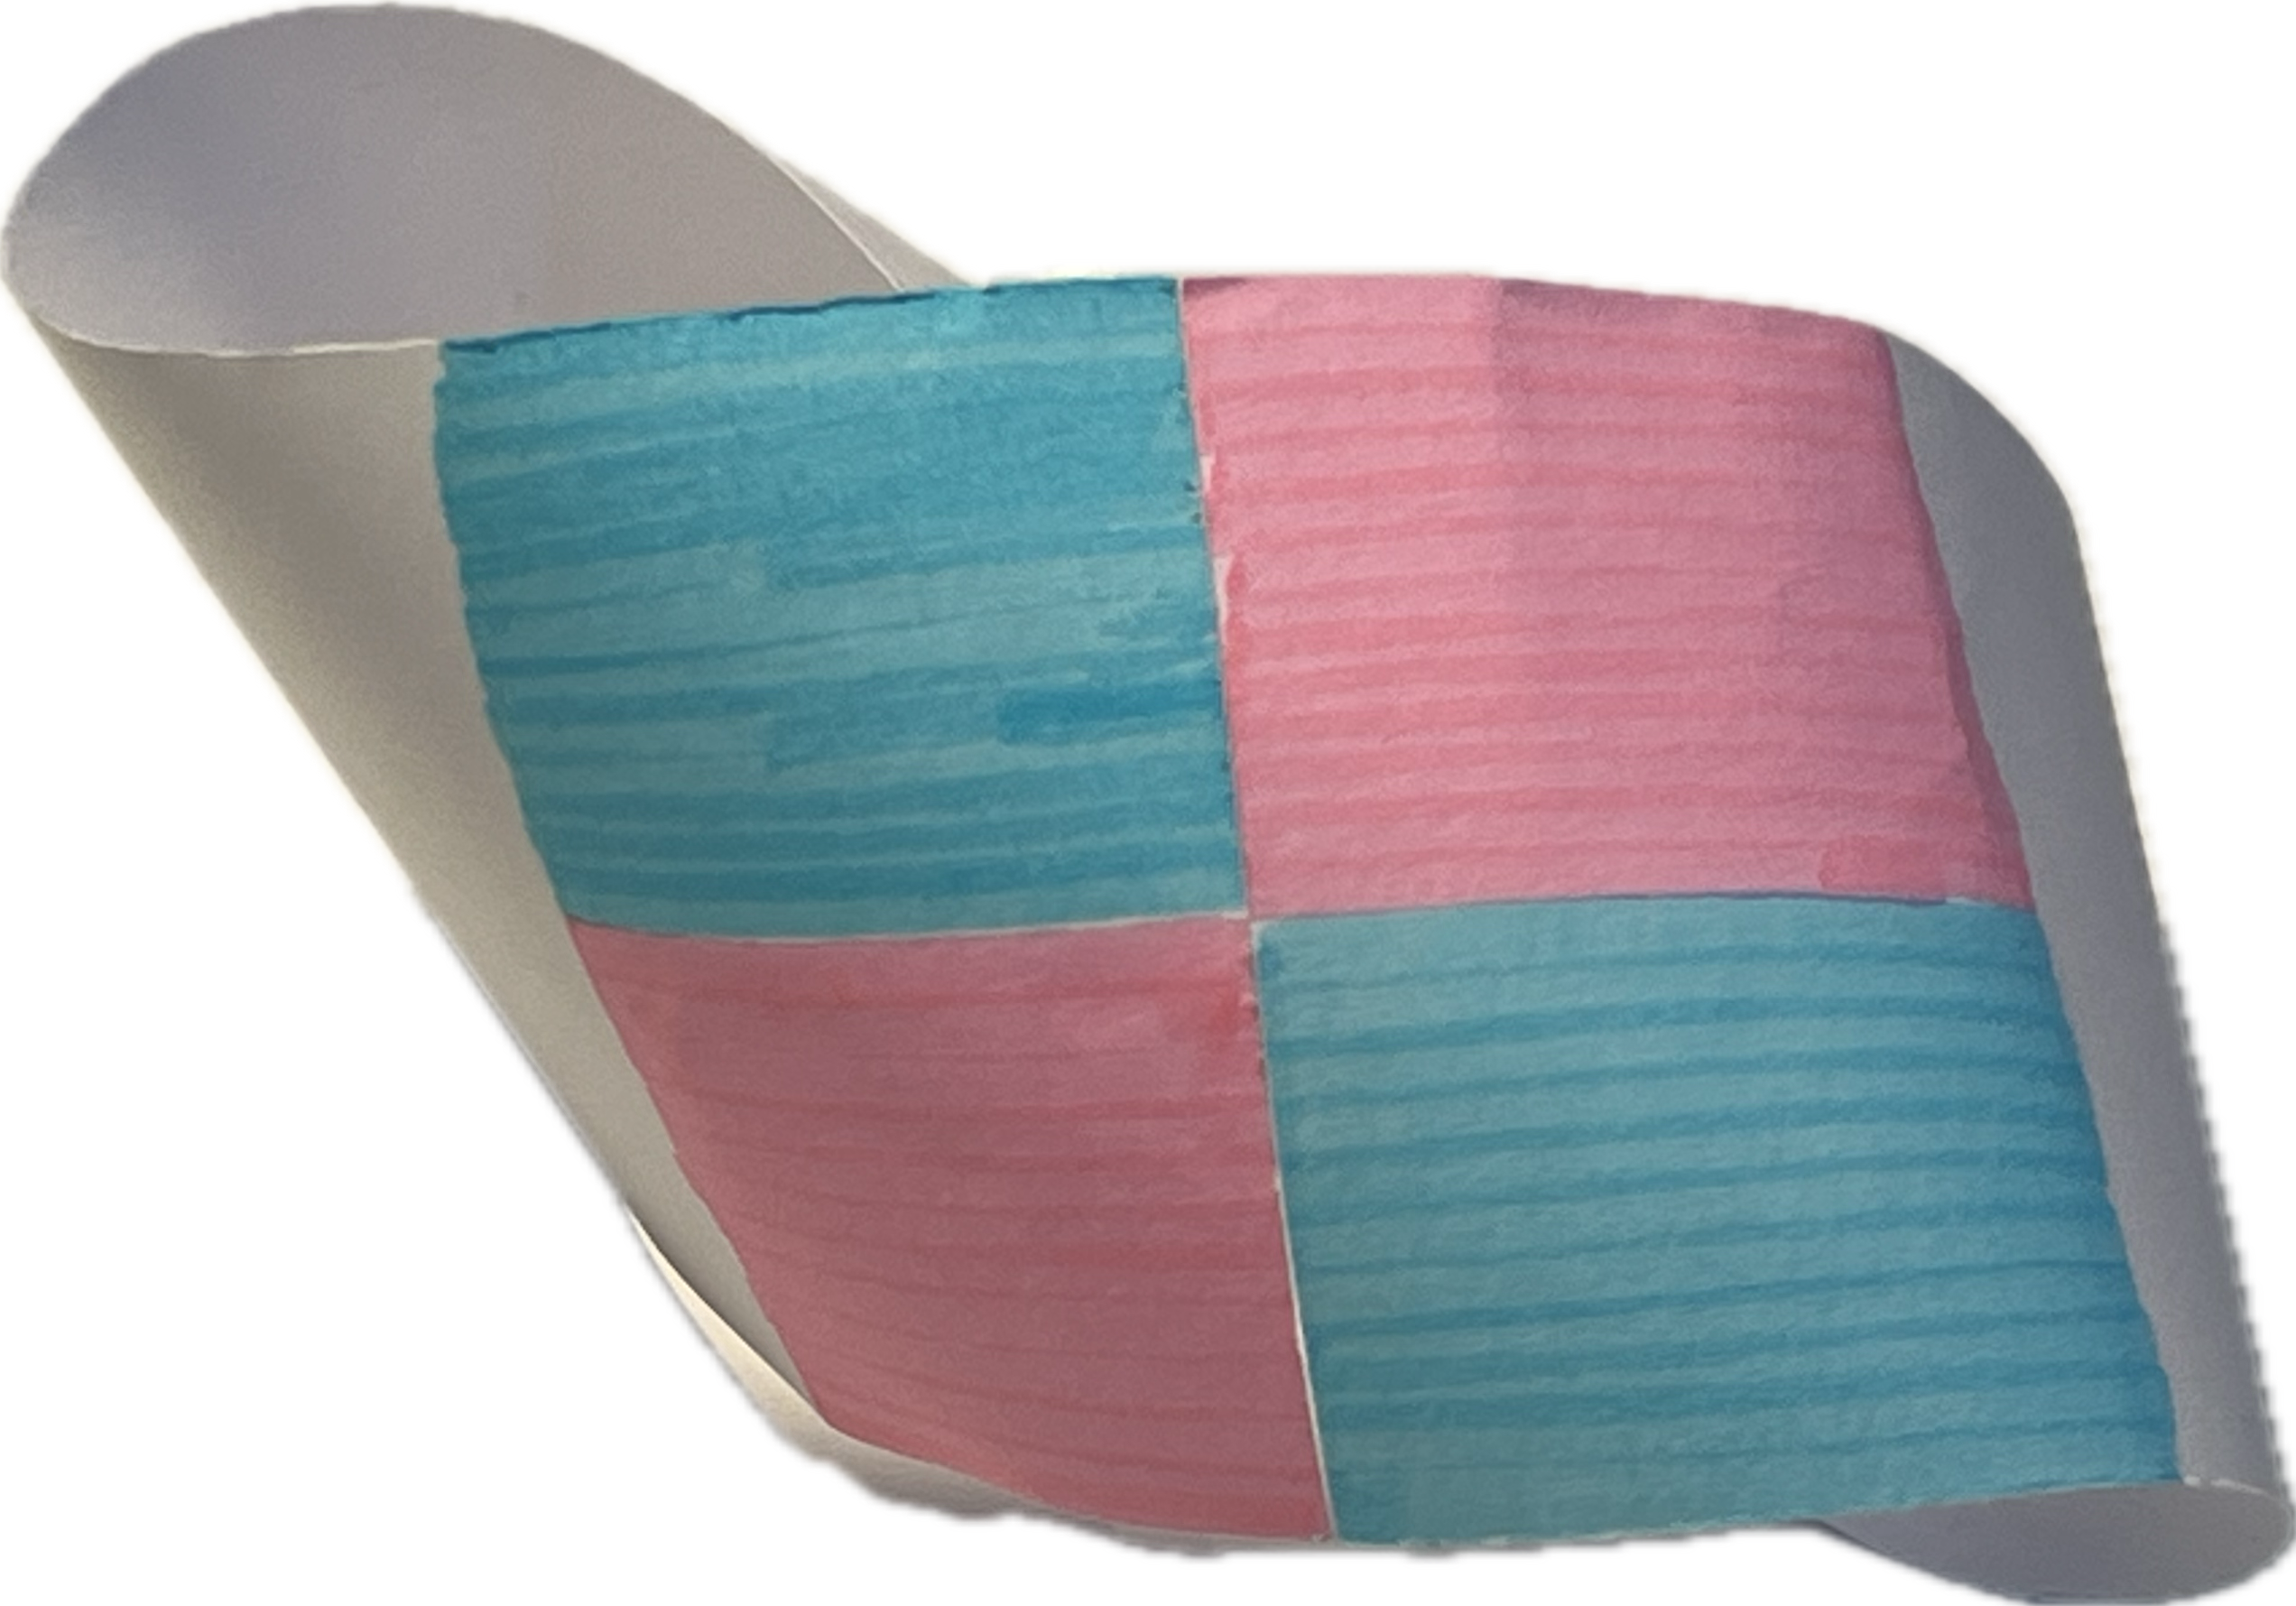
\includegraphics[height=.39\linewidth]{Images/coloured_mobius.png}
      \captionof{figure}{A M\"obius loop with the two connecting ends coloured, showing how the ``left and right side'' join when twisted}
      \label{fig:test2}
    \end{minipage}
    \end{figure}


\subsection*{Evaluation}
The focus on the process of discovery and creativity in this session relieved a lot of pressure from the students. They showed excitement in constructing and manipulating the M\"obius strips. The introduction of crafts into the session did have an impact on the focus of the students, noticeably at the end of the session it was difficult to gather the students' attention.

\subsection{Session 3/4: Statistics}

While the previous activity focused on intrinsic value, this one --- delivered over two lunchtime sessions --- was designed, amongst other things, to incorporate a utility value intervention. This is finding value in maths because you consider it useful for future or present goals \cite{MAES:2024}. It is worth noting that this may not be as influential to students in a primary school. It is unlikely that students give much consideration to the utility the subjects they study provide, as for the majority of students education mathematics is a mandatory subject. Showing the utility of maths may still be beneficial, however not as much as it may be to GCSE or A-level students.
\par
The second goal of this session was to get students talking about maths with their parents. It has been shown that parental involvement can affect children's mathematics performance by reducing mathematics anxiety \cite{Vukovic01052013}. However other studies have found that children of maths anxious parents learn less maths over the school year and have more maths anxiety by the end of the year only if the parents reported helping frequently with maths homework \cite{Maloney:2015}. As a result of this, involvement of parents was aimed to be based around discussion rather than maths questions.
\par
The topic of statistics was chosen as it is on the national curriculum, so the students should have seen it before, and it offers many real world applications for the students to explore. This activity was split over two sessions so the students could collect data in between the sessions to use in the second session. The majority of the first session was spent discussing what statistics is and why it is useful. This conversation was guided but allowed follow the students' interests. It was important to involve student-centred discussion as this aligns with a constructivist approach, which as discussed before can alleviate anxiety \cite{Finlayson:2014}
\par
 The students were then presented with a sheet for collecting data on hair colour, eye colour and age as shown in Figure 3. 
The aim was for students to take these sheets home and to collect data by speaking to their family. The sheet also contained a brief task for the students to research or speak to their parents about a use for statistics, incentivised by a reward of points from a system used in the school. This would hopefully promote discussion with family members and allow them talk about mathematics in a more casual way, without the usual pressure of completing homework questions.
\begin{figure}[htbp]
    \centering
    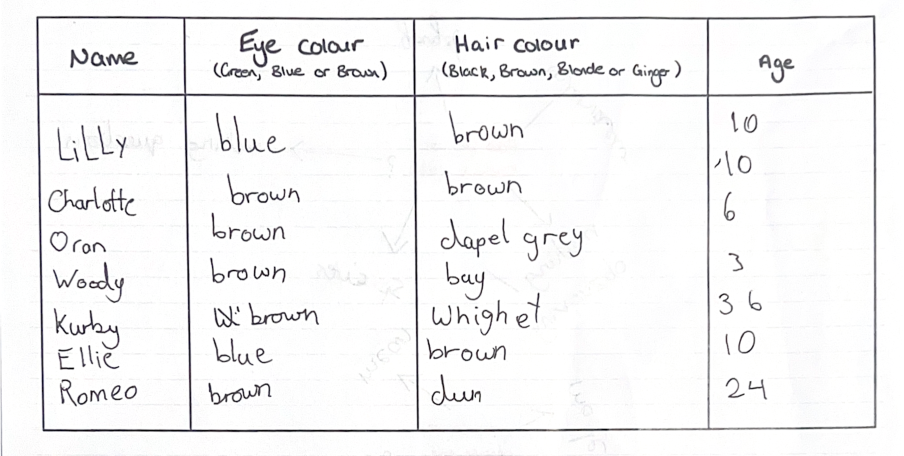
\includegraphics[width=0.5\textwidth]{Images/data_collection_example.pdf}
    \caption{Example of a student's complete data collection sheet, used for the statistics activity}
\end{figure}

\par
\vspace{1em}
The second session focused on the students analysing the data they had collected, this was to be done through the students drawing bar charts and working out averages. A sheet of fake data was created for students who forgot their sheets. The session started with the students using examples of bar charts to see that they are easier to interpret than a table of data. The students then constructed their own bar charts for hair and eye colour (see Figure 4) on a sheet designed to offer guidance. This task was completed more quickly than anticipated, so the session was adapted to introduce the concept of the  median. The girls lined themselves up in age order, and then the middle student was taken as example of a median of their ages. This again links to a constructivist approach to teaching, deviating from a traditional delivery method, with the students themselves being a primary material to learn from.

\begin{figure}[htbp]
    \centering
    \includegraphics[width=0.45\textwidth]{Images/bar_chart_example.pdf}
    \caption{A Bar chart created by a student, representing hair colour data collected previously}
\end{figure}

\subsubsection*{Evaluation}
This task failed to meet the desired aims in two main ways: the mode of delivery and promoting discussion around maths. Due to this session being focused on utility value, this meant trying to fit a larger amount of content into the sessions, and falling back to a more traditional delivery style. Specifically there was one authoritative role in the classroom and although sessions were discussion based the students were still completing worksheets. One student exclaimed ``Ughh, not a worksheet" at the beginning of the first session. This shows how much a traditional delivery style is linked to maths anxiety or at least a lack of enjoyment.
\par
A large aim of this session was promoting discussion around maths with parents and family members through data collection and researching statistics. As the data the students had to collect was so trivial (hair colour, eye colour and age), the students simply recalled the information and wrote it down on the sheet without speaking to anyone. Although some students showed interest in finding uses of statistics at the end of the first session, none of them completed any research on their own. The vast majority of students either lost the data they collected or forgot to bring it in, this means any motivation provided by the students working on their own data was lost.
\par
The rest of the sessions were designed to be self-contained and to avoid overlapping with traditional delivery methods where possible.

\subsection{Session 5: Coordinate Grid}
With the limitations of the previous sessions in mind, it was important that the mode of delivery for this activity was different. All previous sessions had taken place with the students sitting around a group table, so this activity was designed to allow greater freedom of movement in the students. Until now the students hadn't worked collaboratively, as much as they hadn't worked towards one goal or shared this answers. One study suggests that ``incorporating cooperative groups in problem-solving situations, where pupils, given a  variety of problems; work together and share their solutions" helps to reduce maths anxiety \cite{Alkan:2013}. When students collaborate on different problems towards a common goal, they may not worry about competing with their classmates as much as if they were all answering the same questions. Moreover, it has also been found that ``girls are more likely to learn in cooperative mathematics activities'', as girls utilise words more in the learning process than boys \cite{Hughes:2006}.
\par
The content of this session would be a mixture of something new in the form of the coordinate grid, combined with revision of content the students had covered in the previous weeks. This would hopefully make the students feel comfortable as they feel more confident when they see material they have already covered. To begin with the students were introduced to the coordinate grid, and told how to read off a point from the grid. Before the session began, a coordinate grid --- where each point was a piece of paper --- was laid out on the floor. On the back of some of the pieces of paper were questions on topics the students had recently covered (see appendix A). Each correct answer directed students to the next grid point and corresponding questions, revealing where a prize was hidden along the way. It was required that each student solve at least one question to get the prize at the end. 
\par
The design of this session directly aligns with the theory mentioned earlier, students are solving problems individually but have to share their answers to find the next question. There were also instances where students collaborated on more difficult questions, this promoted a cooperative environment.


\subsubsection*{Evaluation} 
The form of this session worked well at reducing anxiety in students. Every time a new clue was discovered, students were asked who would like to complete it, all the students who hadn't completed a clue yet volunteered. This is not something you would see happen during a normal lesson, with students previously stating that they are worried about other classmates judging them. As the students were working towards a common goal they do not have to worry about other students judging them, as it benefits the other students if everyone is supported and does well.

\subsection{Session 6: 1-2 Nim}
While the previous activities had used some constructivist approaches to teaching, for this session it would be the main focus. One study of 12-year-olds found that the difference in maths anxiety of those taught with constructivist approach against a control group was significant at a level of 0.01 \cite{Suman:2021}. Moreover, when looking only at girls, the difference was more significant (i.e. a higher t-value) than when looking at only boys or a mixed group. However, this study fails to mention the specifics of the constructivist approach that was adopted, so it is not possible to recreate these results directly. 
\par
The approach used in the following activity is ``Discovery Learning" first outlined by Jerome Bruner \cite{Bruner:1961}. Discovery learning takes place in a problem-solving environment where students draw on previous knowledge and manipulate objects to discover new facts and relationships \cite{learning-theories:Discovery-learning}. This session was based around the game ``1-2 Nim" taken from the math for love website \cite{1-2Nim}, the aim was for students to discover their own strategies for the game. The simplest version of this game involves two players and eight counters, students take turns taking either one or two counters and the student to take the last counter wins. An example of a game of 1-2 Nim is shown in Figure 5.
\par
\begin{figure}[htbp]
    \centering
    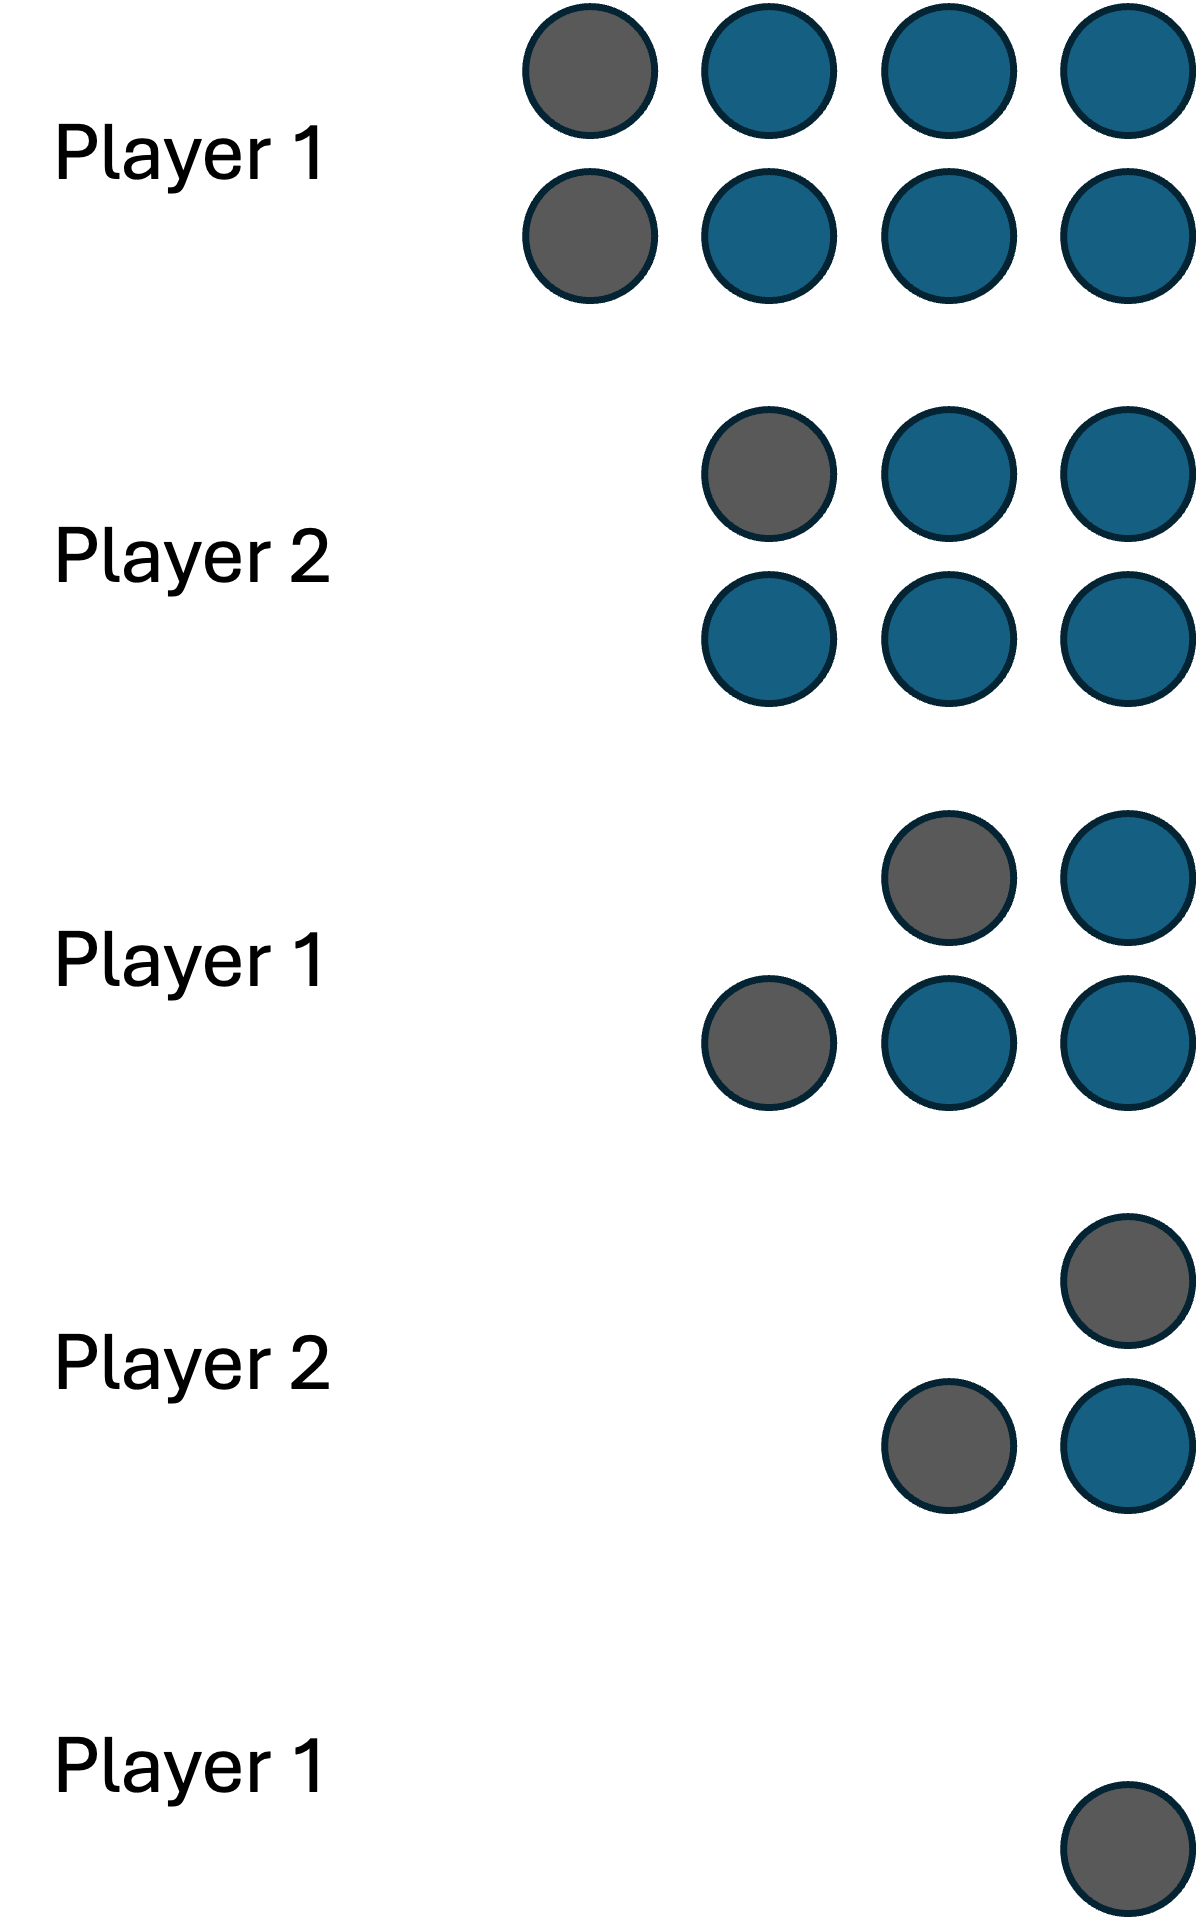
\includegraphics[width=0.25\textwidth]{Images/1-2Nim_example.png}
    \caption{Example of a game of 1-2 Nim}
    \end{figure}


This game was demonstrated by playing against a student until it was clear everyone understood the game. The students were then invited to play against each other, this allows them to explore the game without any extrinsic goals. Following this, students were then brought back to use a powerful problem-solving technique to start discovering strategies, they were asked how we could make the game simpler. With some guidance students then discussed the trivial strategy for playing with one or two counters and then the slightly more difficult case of three counters (here you wish for your opponent to take first). For the rest of the session the students were left to play against each other to discover the best strategy for four to eight counters. While constructivism and discovery learning does not mean you should never tell students anything directly, in this activity this was the case. Students conjectured strategies which were tested by playing against other students or myself. The students organised this information by creating a table of their strategy for each number of counters. An example of a strategy table produced by a students is shown in Figure 6. By creating and using their own strategy tables, students demonstrated genuine ownership of the learning process.

\begin{figure}[htbp]
    \centering
    \includegraphics[width=0.9\textwidth]{Images/1-2Nim_strategy.pdf}
    \caption{Strategy sheet created by a student to record optimal moves in the 1-2 Nim game}
\end{figure}

\subsection*{Evaluation}
The combination of the competition of the game and Discovery Learning acted as a powerful motivation tool for the students. Students who didn't necessarily lack in confidence but were simply disinterested now were keen to take part in the session and  volunteer answers. Figure 6 shows how the students were able to grasp the strategy of the game and effectively extrapolate to a game with a higher number of counters.
\section{Evaluation}

\subsection{Consideration of Original Aims}
Due to the nature of the project aims, it was difficult to elicit quantitative evidence. It was deemed inappropriate to ask students to self-report their levels of maths anxiety, as doing so could have risked increasing anxiety or making students more self-conscious. Therefore, the evaluation of the project relies primarily on observations and qualitative feedback.

\subsubsection*{Aim 1 -- Increasing self-confidence in girls in maths}
As the sessions progressed it was observed that the girls became more willing to contribute. In the first session the students tentatively raised their hands when they were asked questions and as sessions went on students were so eager to contribute they often spoke over each other. Although this behaviour indicates growing confidence, it is difficult to fully isolate the cause. Part of the increase may reflect students' acclimatising to the small-group environment rather than the specific interventions. 
\par
One notable incident occurred during the first statistics session. When asked about the meaning of ``data'', none of the students initially volunteered an answer. After a few seconds, one student raised her hand and suggested, ``is it information?". Although initially uncertain, the student took the risk of offering an answer. This behaviour is unlikely to have occurred in a regular classroom setting, it is most likely the small group size and possibly the more informal environment that made the student feel more confident. This could also be looked at as evidence of decreased maths anxiety, the student was unsure of themselves but willing to contribute as they are less worried about the consequences of an ``incorrect" answer.


\subsubsection*{Aim 2 -- Decreasing maths anxiety in girls}
The evaluation of this aim presents more challenges. There were still observable instances of anxiety-related behaviours during the project. For example, in the coordinate grid session, students solving problems individually sometimes appeared uncomfortable when being observed by their peers. One student expressed that she disliked others watching her work, indicating a residual fear of judgement. Although the collaborative structure of the session aimed to reduce such pressure, the format meant that one student would be working at a time, placing a lot of pressure on that student.


%It is easier to evaluate the limitations of this project in regards to this aim than it is its successes. Throughout the project there were some examples of students exhibiting behaviour suggesting they may be feeling anxious. In particular the coordinate grid session which involved students working out problems on their own sometimes required them to sit down and spend a minute or two solving the more challenging questions. When one student was sat down solving a question, other students came over to look as they were eager to get through the session. This made the student who was solving the problems nervous, and she said that she didn't like people watching her. This was likely due to a fear of judgement that she would get the questions wrong or she was taking too long to solve the questions. Although this session was designed so the students would be working together, the format meant that one student would be working at a time, placing a lot of pressure on that student. 
\par
A key positive indicator was the students' growing enthusiasm for attending the sessions. As the project progressed, students showed eagerness to attend and expressed disappointment that the sessions would be ending. Although enjoyment is an indirect metric, increased enthusiasm for mathematical activities likely reflects a reduction in anxiety levels. Increased enjoyment is likely caused by the same design choices intended to decrease anxiety, such as using a more constructivist approach and focussing more on the process of learning.

%The most notable proxy for the success of the project in regards to this aim was the enjoyment and the enthusiasm the students exhibited for the sessions. All of the students were eager to turn up to the sessions later into the project, and seemed disappointed that the sessions would be ending. While this is clearly a very loose metric of decreased anxiety, increased enjoyment likely means that the methodology behind the design of the sessions was effective. That is, increased enjoyment is likely caused by the same design choices intended to decrease anxiety, such as approaching a more constructivist approach and focussing more on the process of learning.

\subsection{Limitations}
One major limitation of this project was highlighted by a comment made by as student during the final session: ``I enjoyed you sessions but I still don't like maths lessons". This suggests that no matter how successful the sessions were at decreasing anxiety it is difficult to transfer this to a regular maths lessons.
\par
 Addressing this issue could involve providing teacher training on some of the methods outlined to help produce a classroom environment which reduces maths anxiety. Another possible approach is to treat the causes of anxiety, this could be done through identifying and changing negative beliefs. Two methods supported in the literature are expressive writing and bibliotherapy \cite{MAES:2024}. Expressive writing involves students writing freely about events that provoke anxiety, while bibliotherapy encourages them to read about and reflect on relatable challenges. Both approaches are suitable for a classroom setting and offer potential for longer-lasting benefits compared to lesson design changes alone.
 

\subsection{Legacy and Conclusion}

The legacy of this project lies not with the physical materials, but in the students attitude and perception of mathematics. During the final session, a more direct discussion on self-confidence was held, recognising the students' hard work and their demonstrated potential in mathematics. It is anticipated that even a small positive experience with maths, such as this project, will stay with some of the students and inspire them in the future.
\par
Overall, this project has demonstrated the extent to which carefully planned, student-centred lesson design can alleviate aspects of maths anxiety and support the development of confidence. However, it has also shown that a holistic approach --- including learning environment, teacher practises and direct intervention targeting beliefs and attitudes --- is required to address maths anxiety and self-confidence comprehensively.


\bibliographystyle{unsrt}
\bibliography{bibliography}

\clearpage

\appendix

\section{Sample of Questions used in coordinate grid session}
\begin{figure}[htbp]
    \centering
    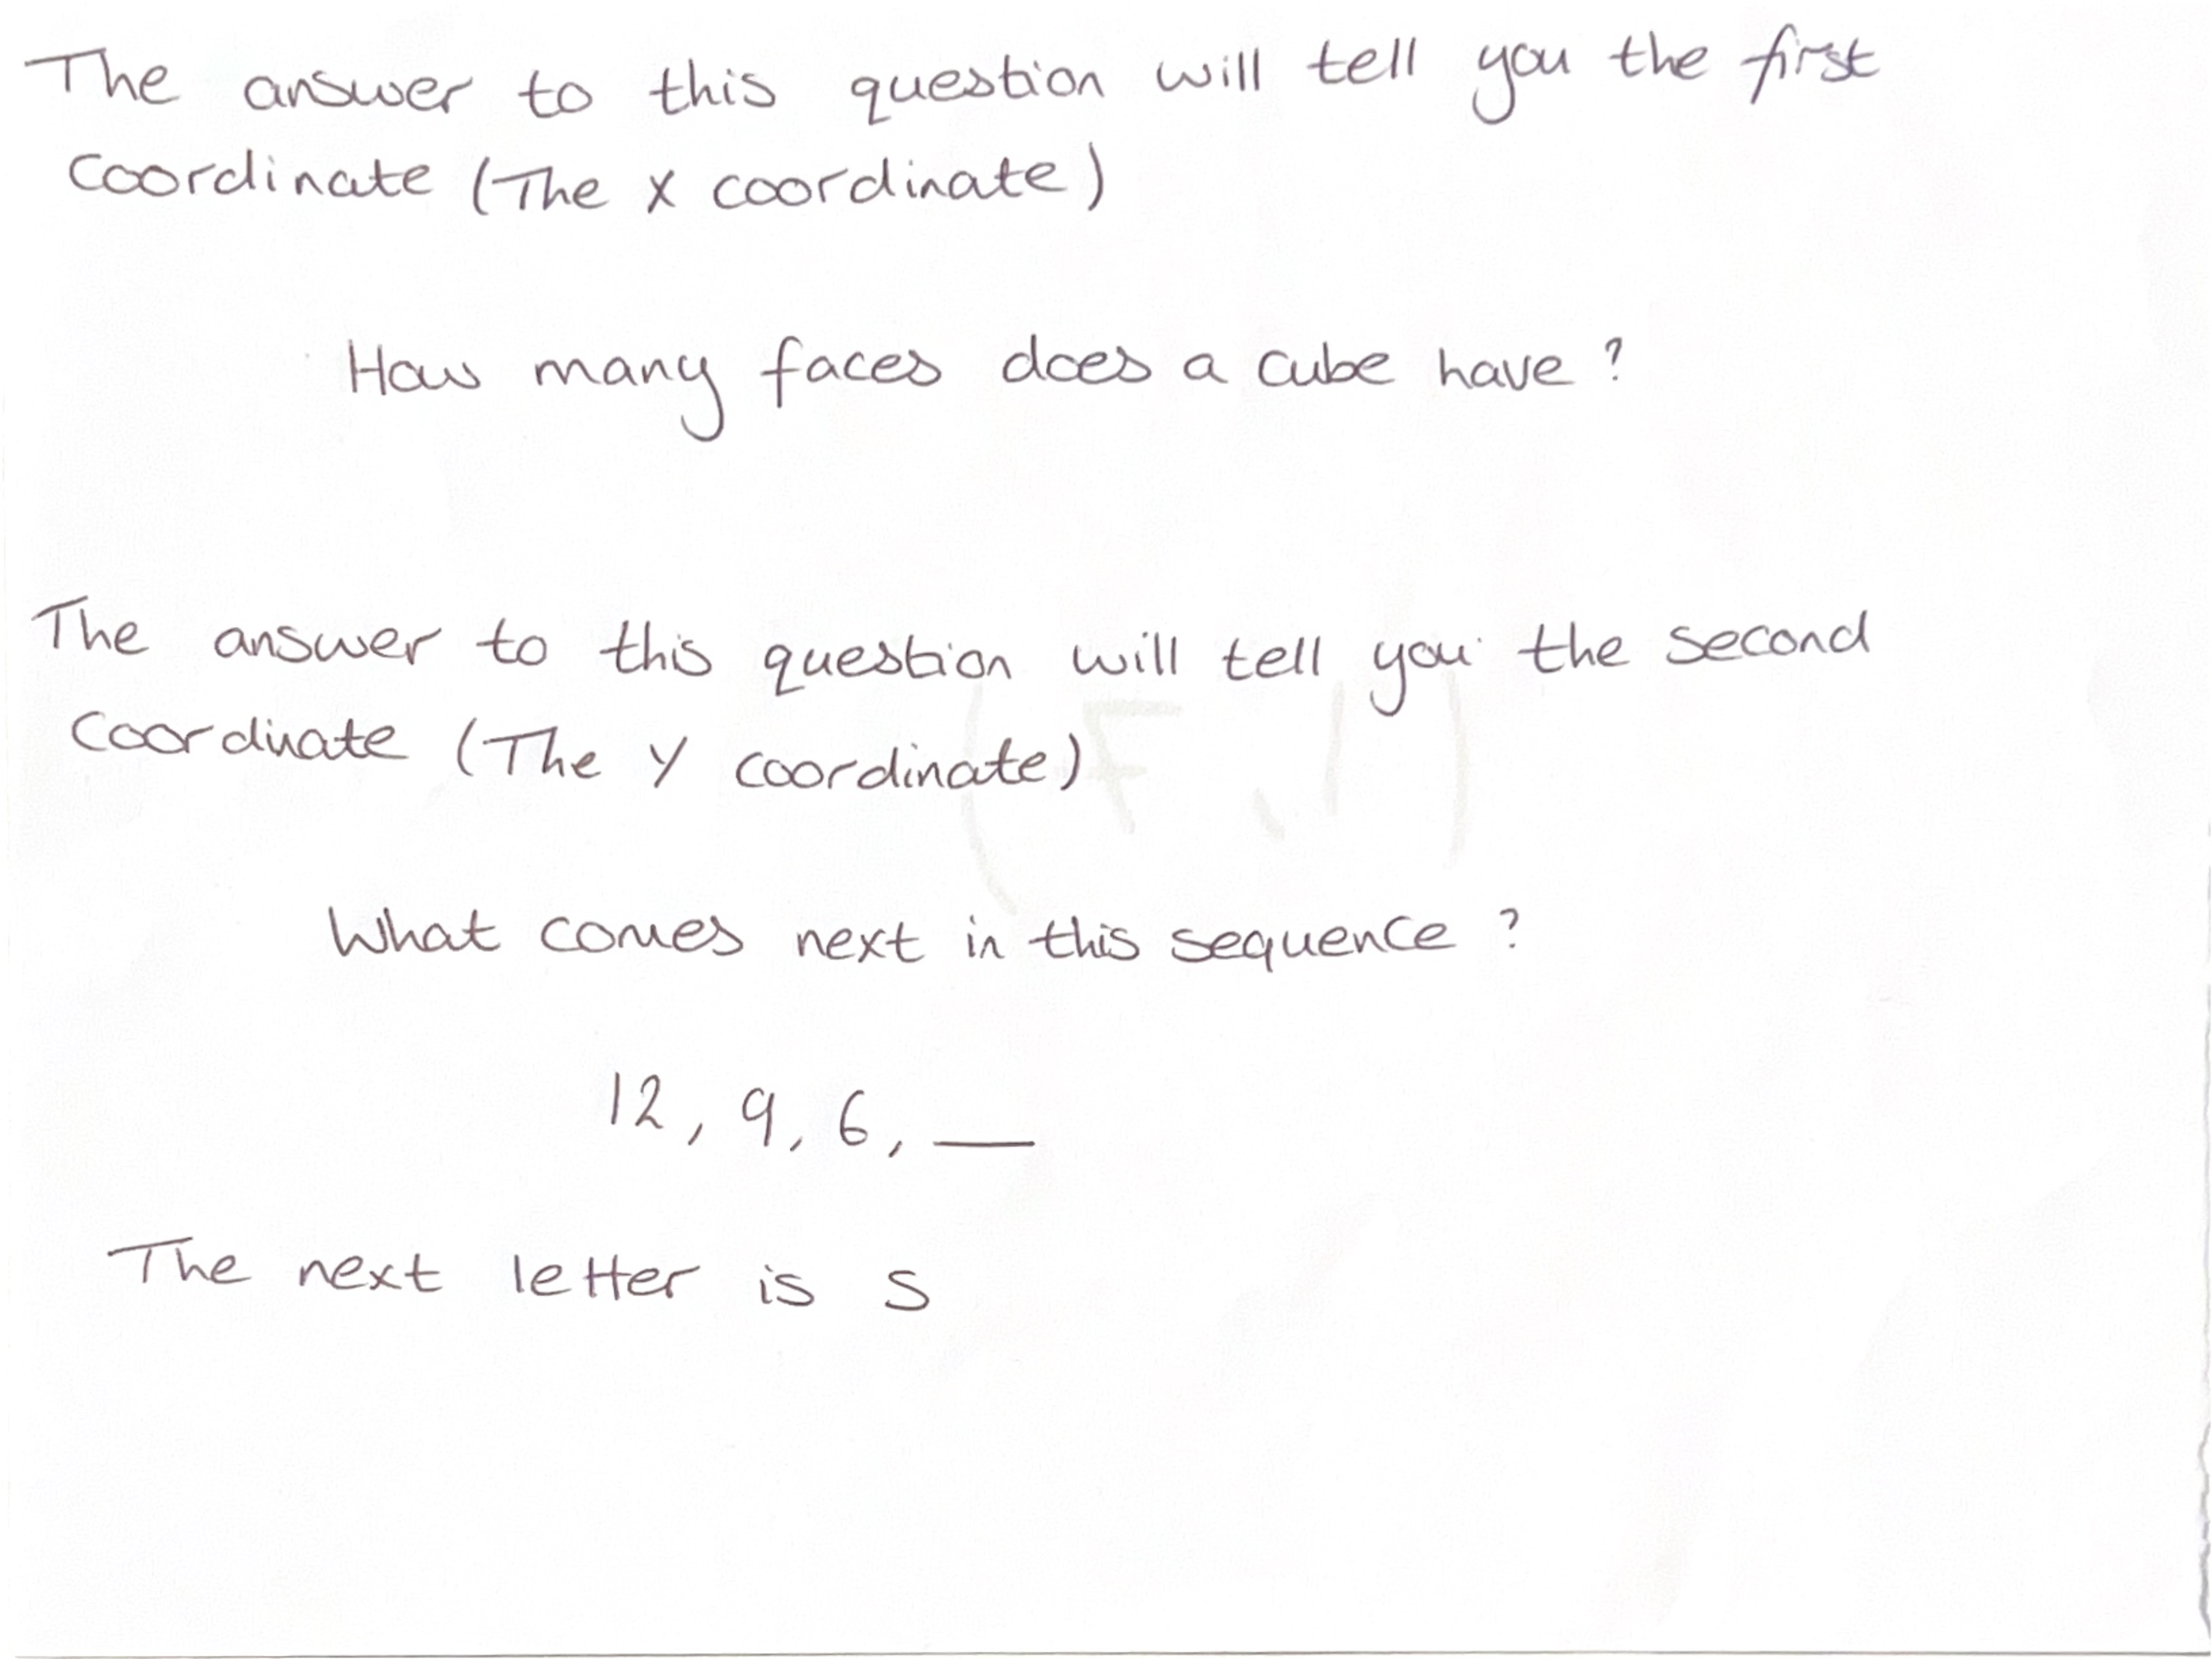
\includegraphics[width=0.9\textwidth]{Images/CoordinateGrid_questions-pages-1.pdf}
\end{figure}
\begin{figure}[htbp]
    \centering
    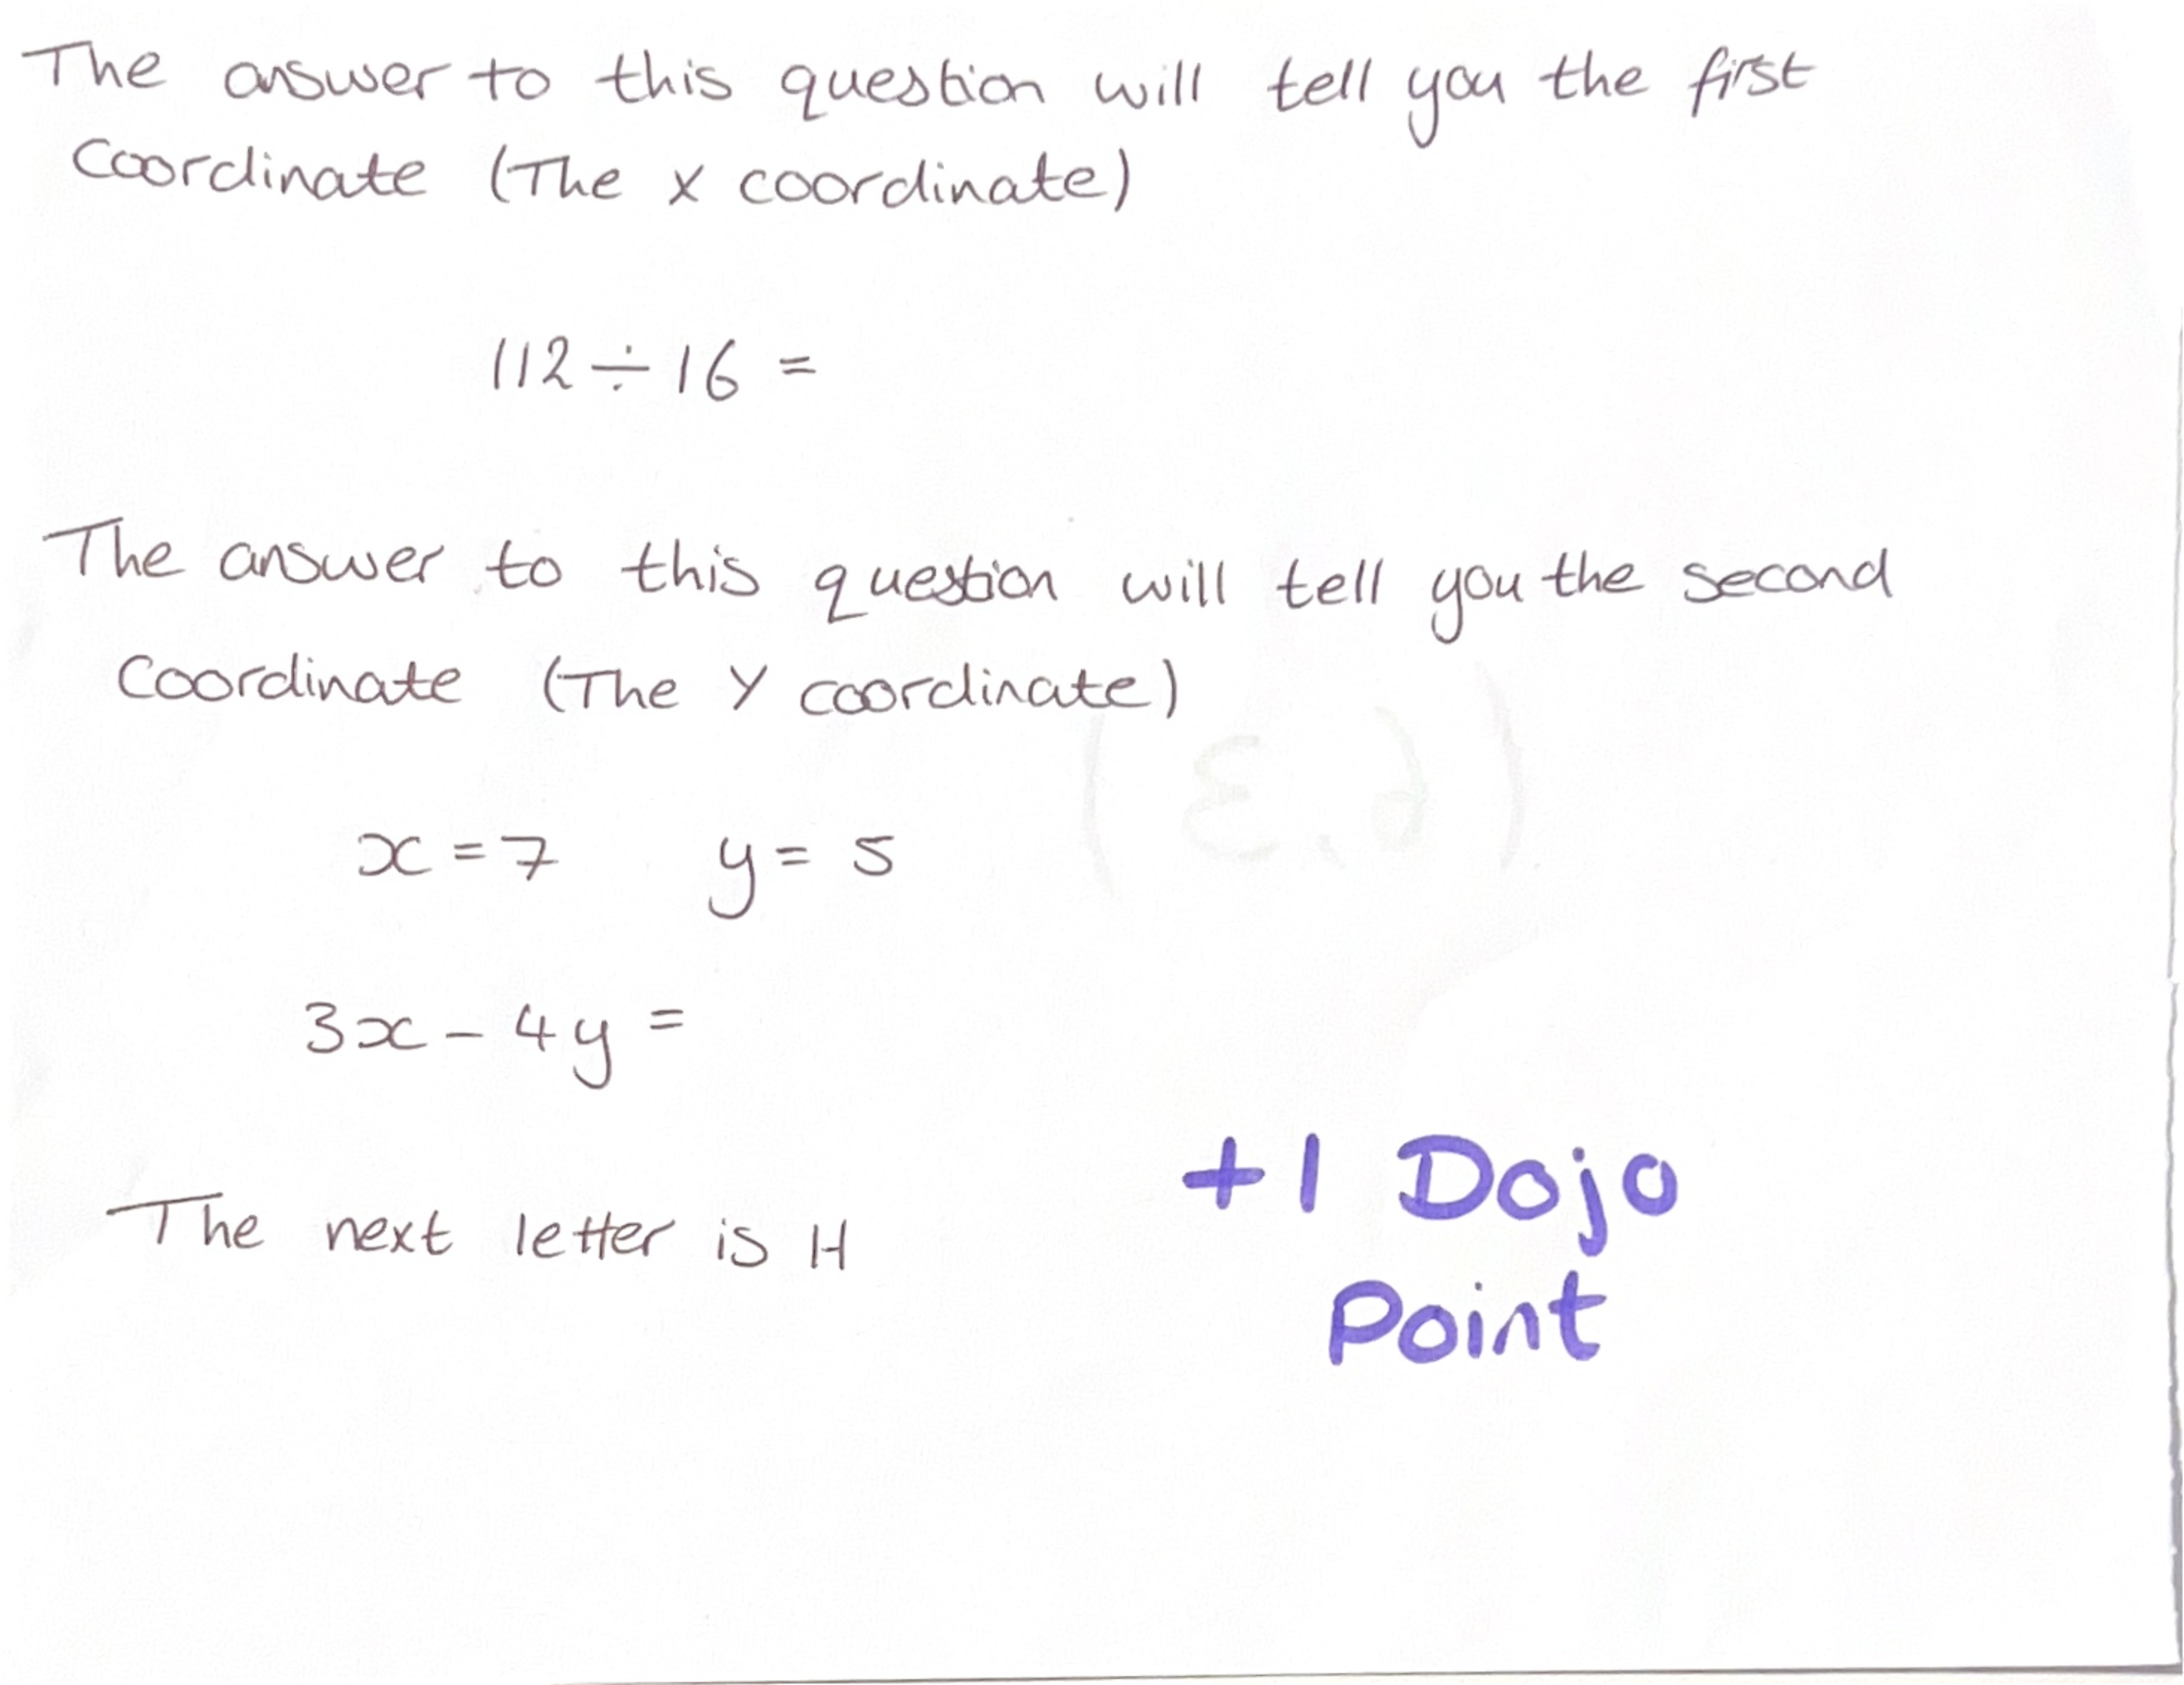
\includegraphics[width=0.9\textwidth]{Images/CoordinateGrid_questions-pages-2.pdf}
\end{figure}
\begin{figure}[htbp]
    \centering
    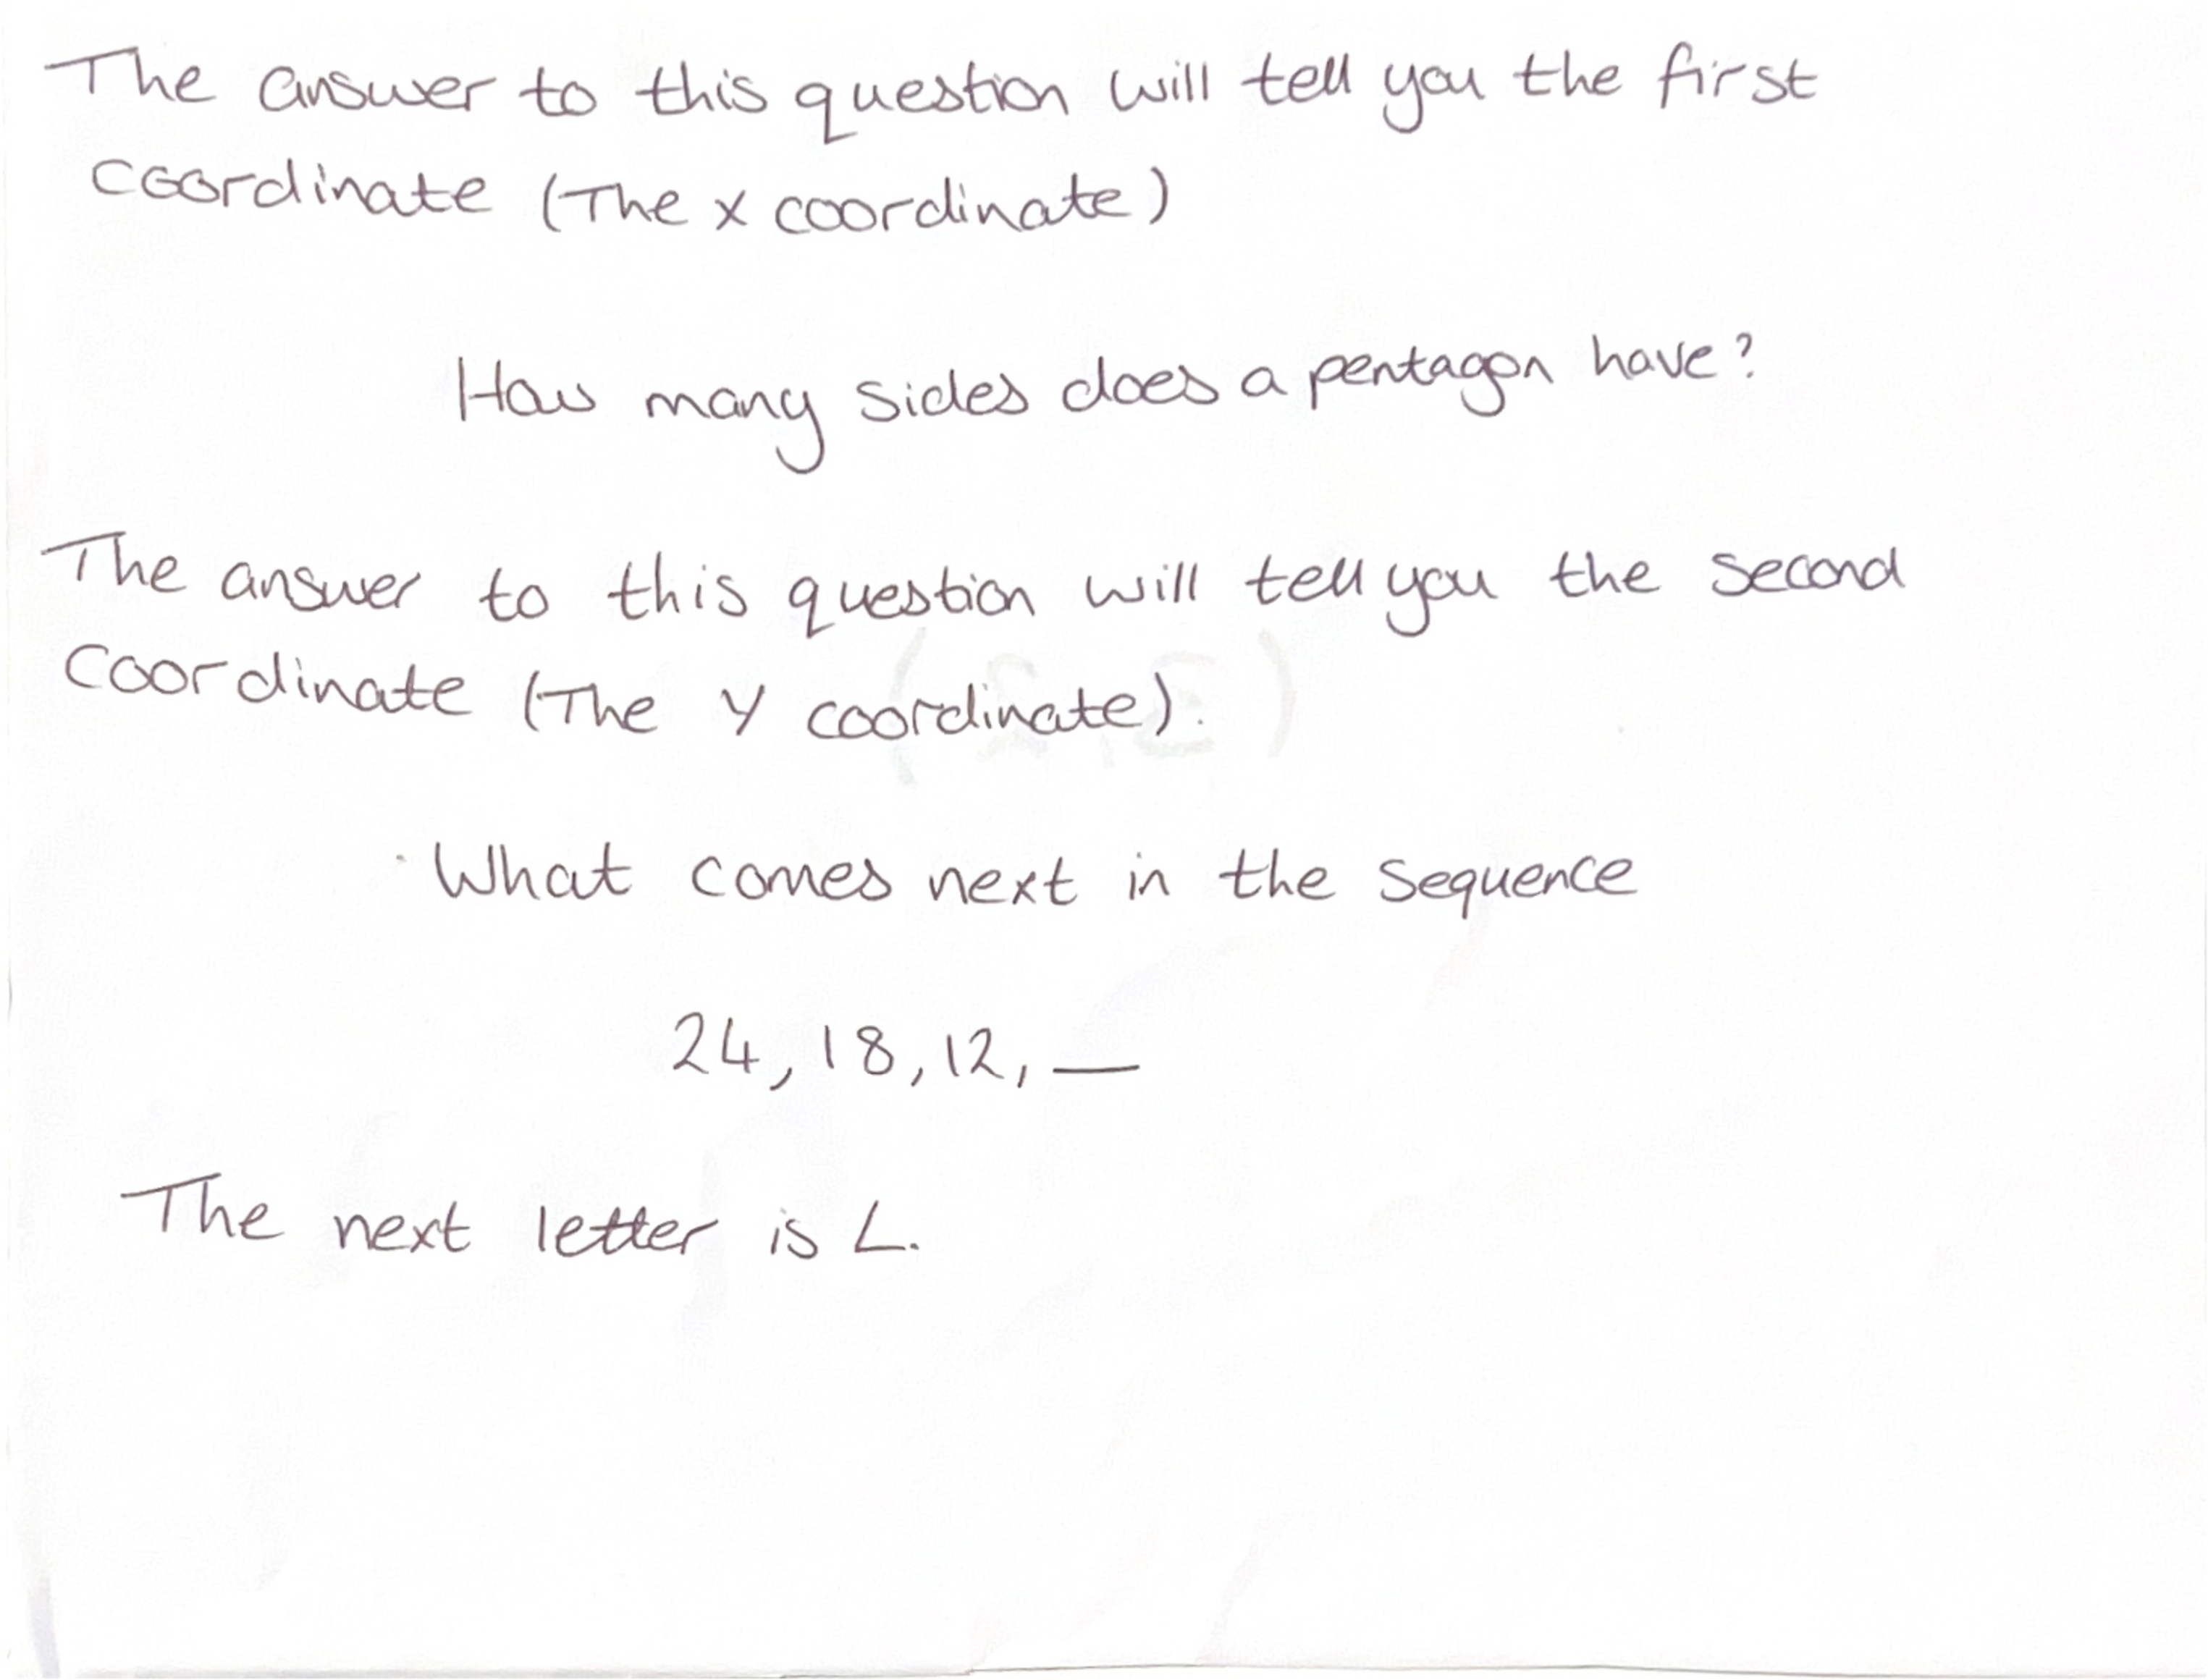
\includegraphics[width=\textwidth]{Images/CoordinateGrid_questions-pages-3.pdf}
\end{figure}
\begin{figure}[htbp]
    \centering
    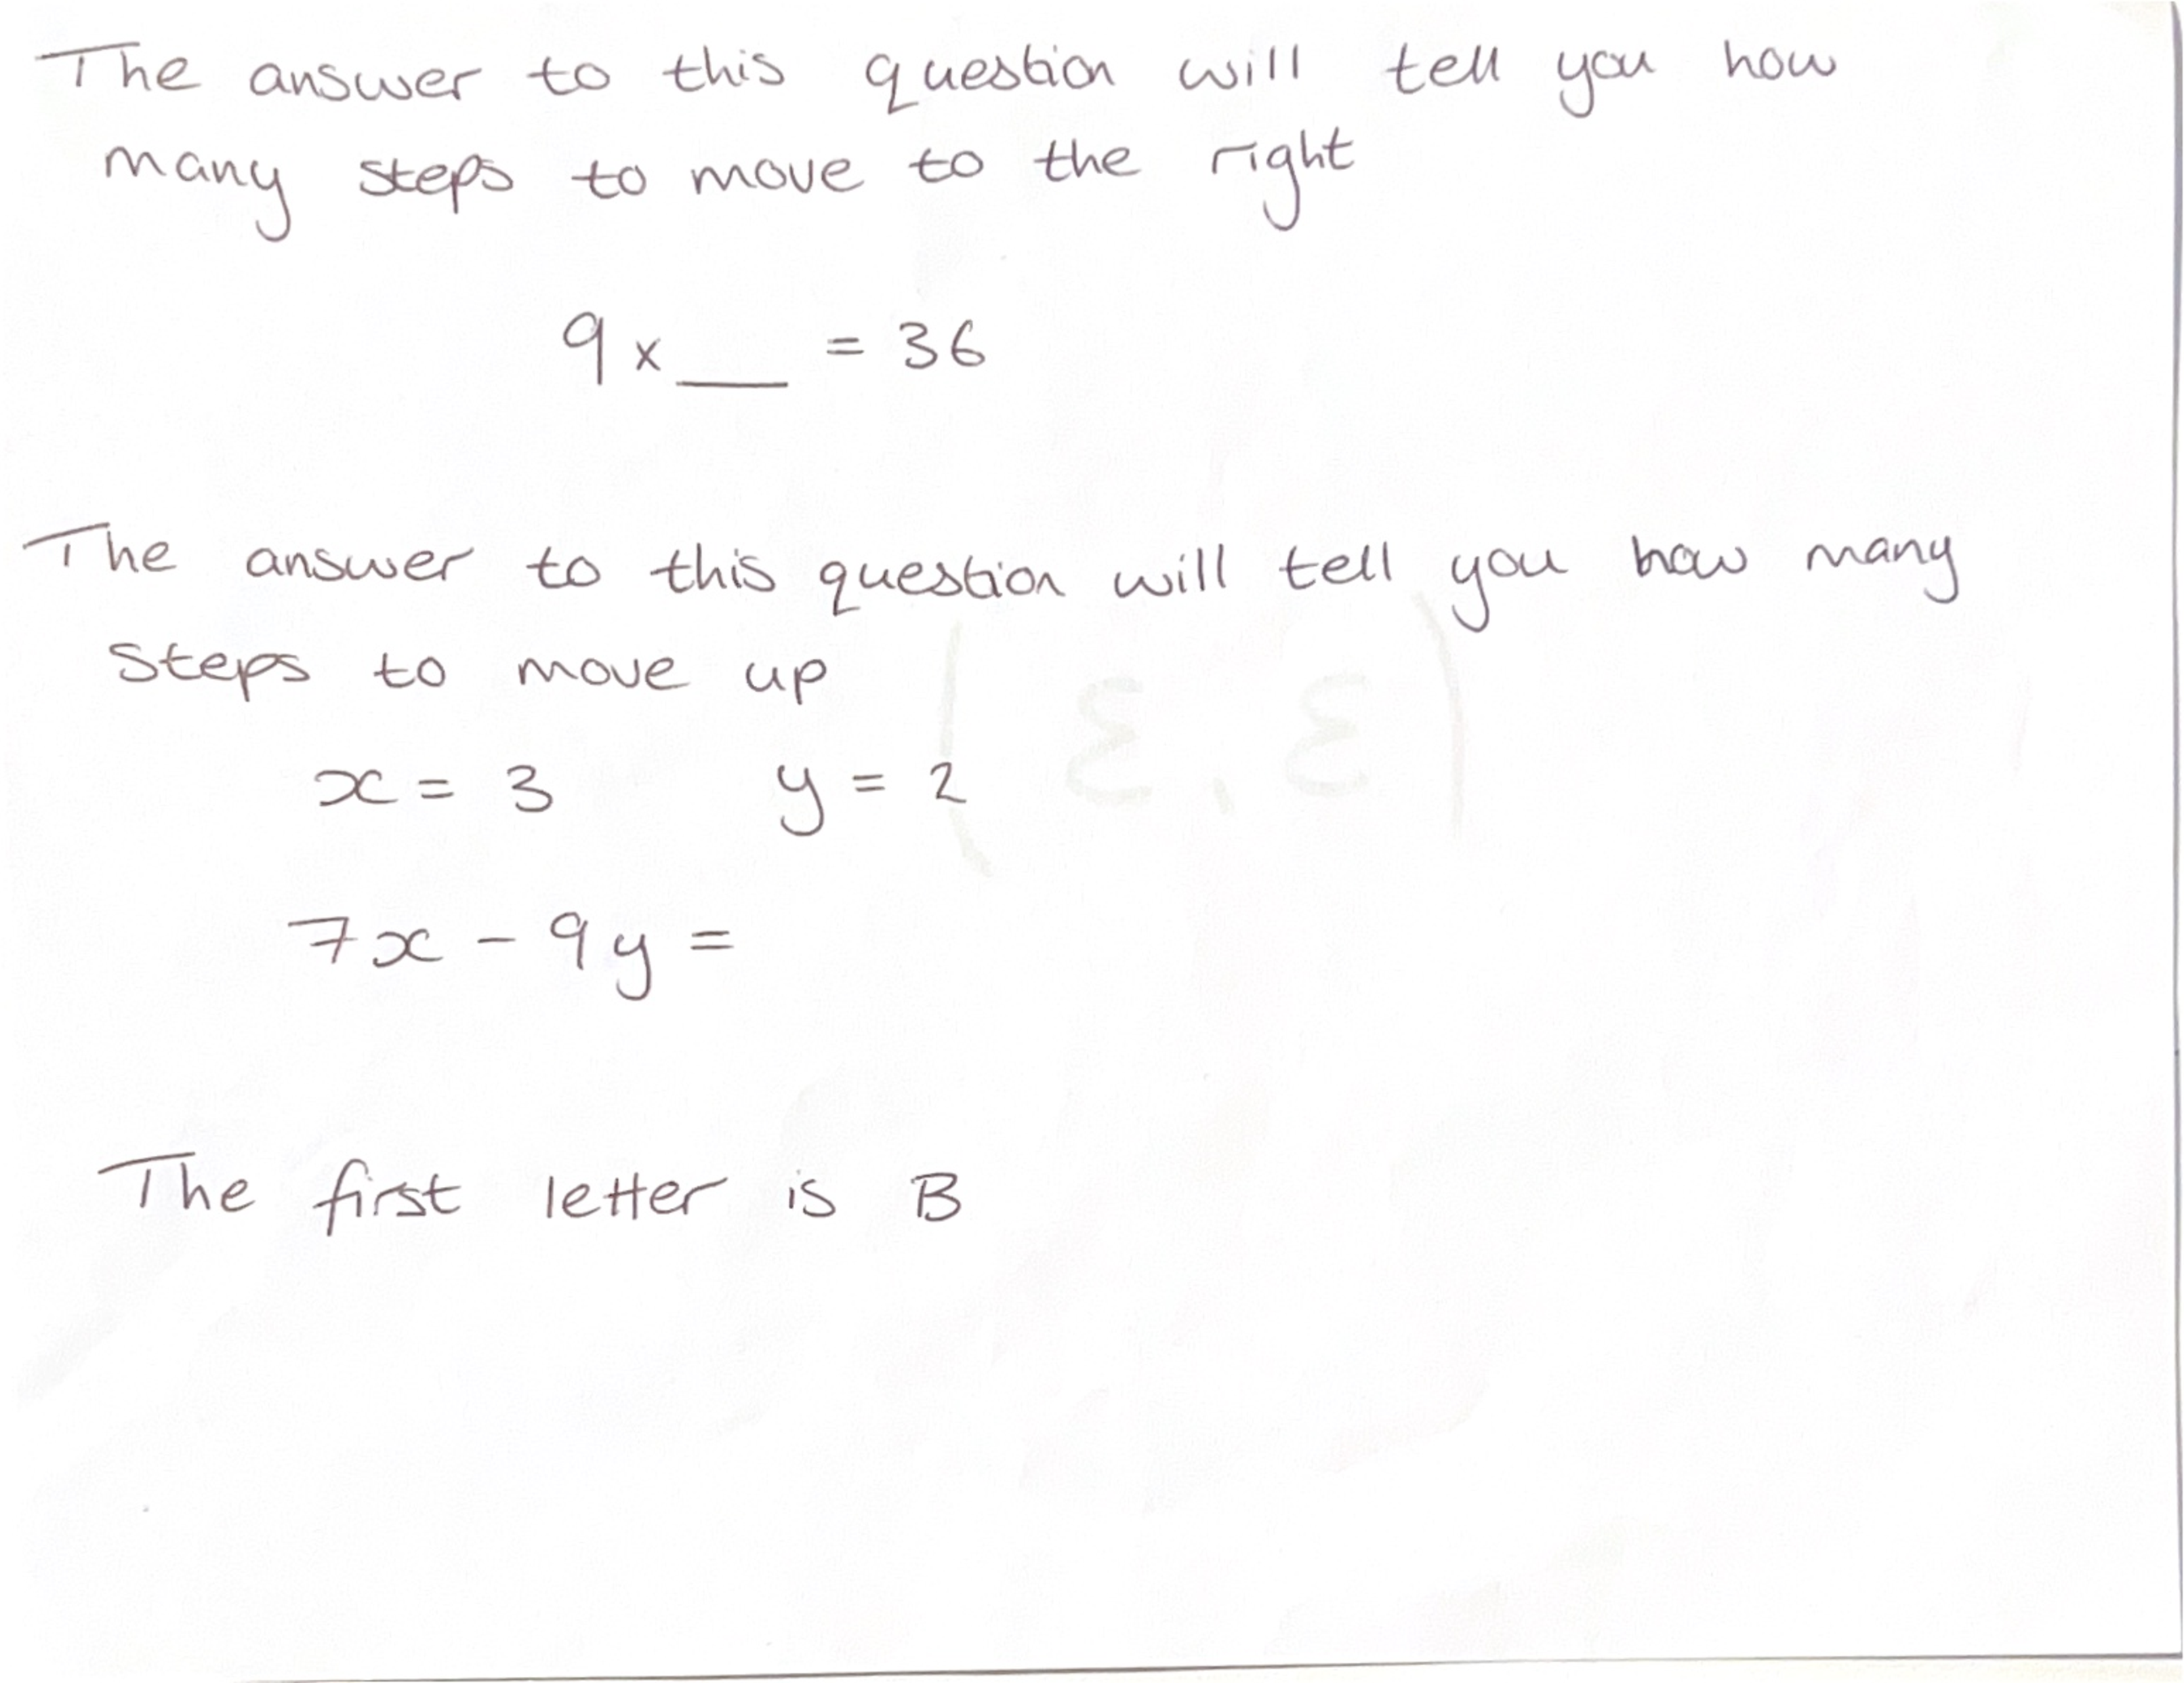
\includegraphics[width=\textwidth]{Images/CoordinateGrid_questions-pages-4.pdf}
\end{figure}
\begin{figure}[htbp]
    \centering
    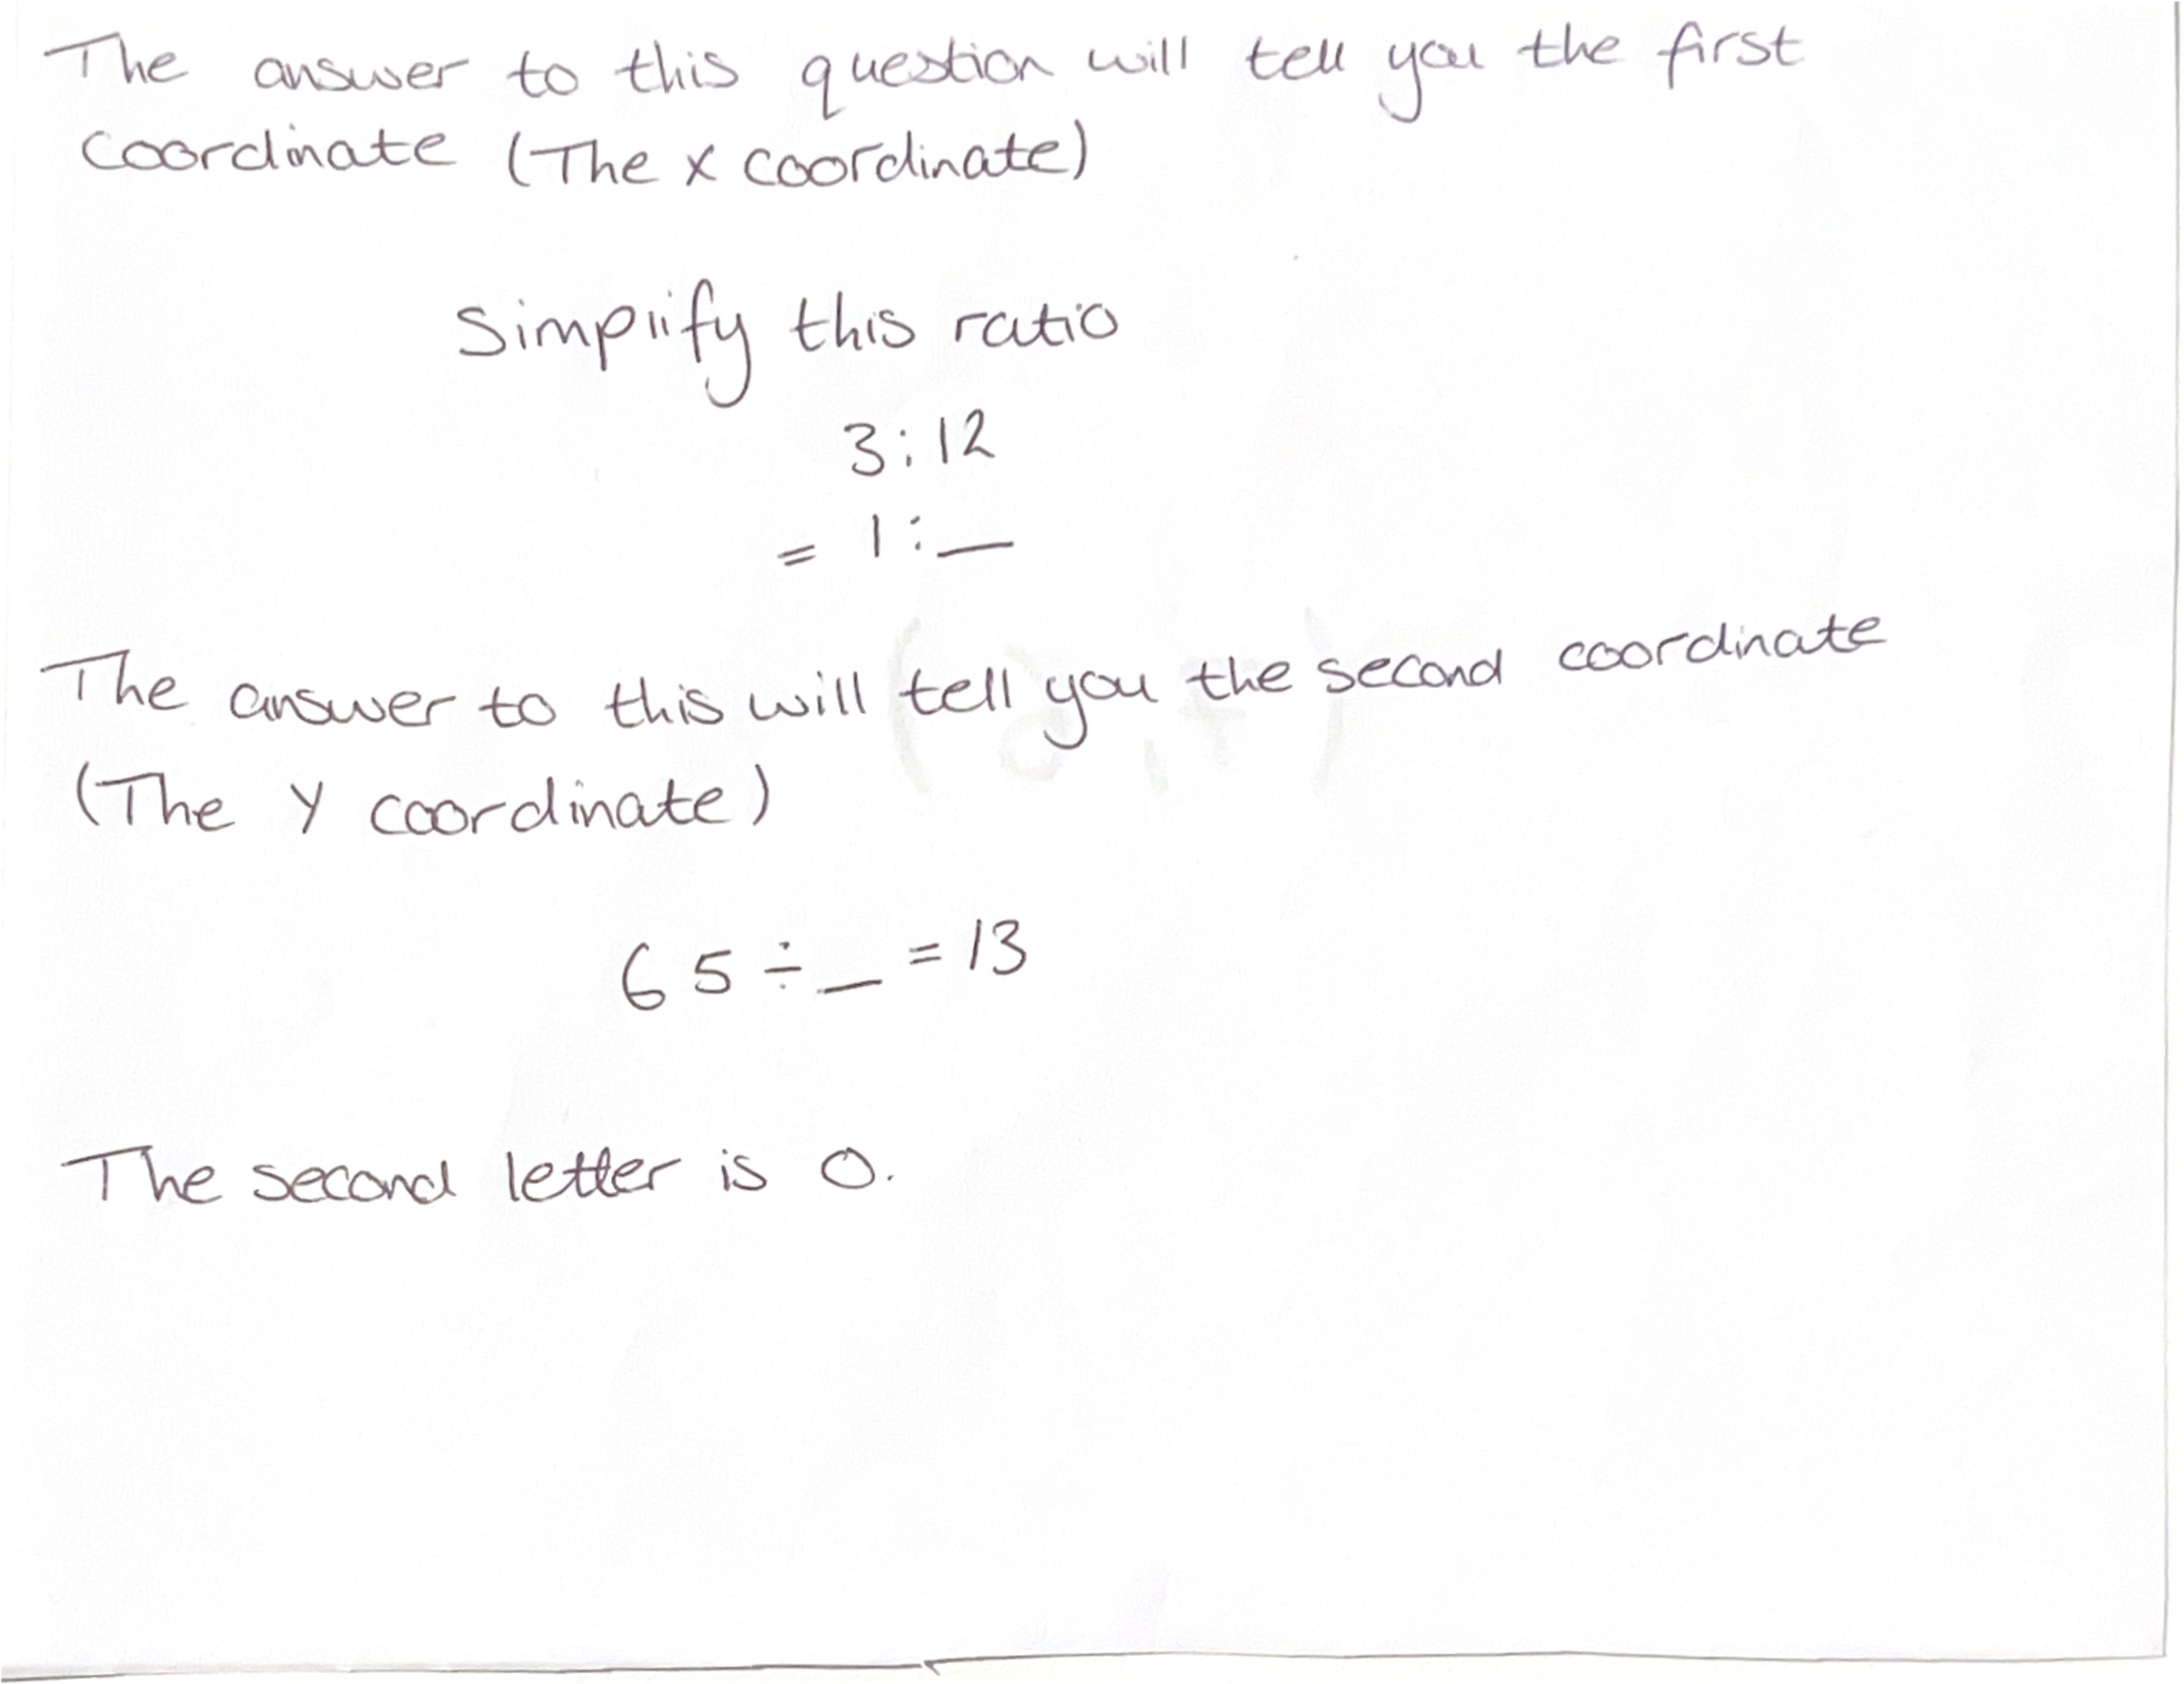
\includegraphics[width=\textwidth]{Images/CoordinateGrid_questions-pages-5.pdf}
\end{figure}
\begin{figure}[htbp]
    \centering
    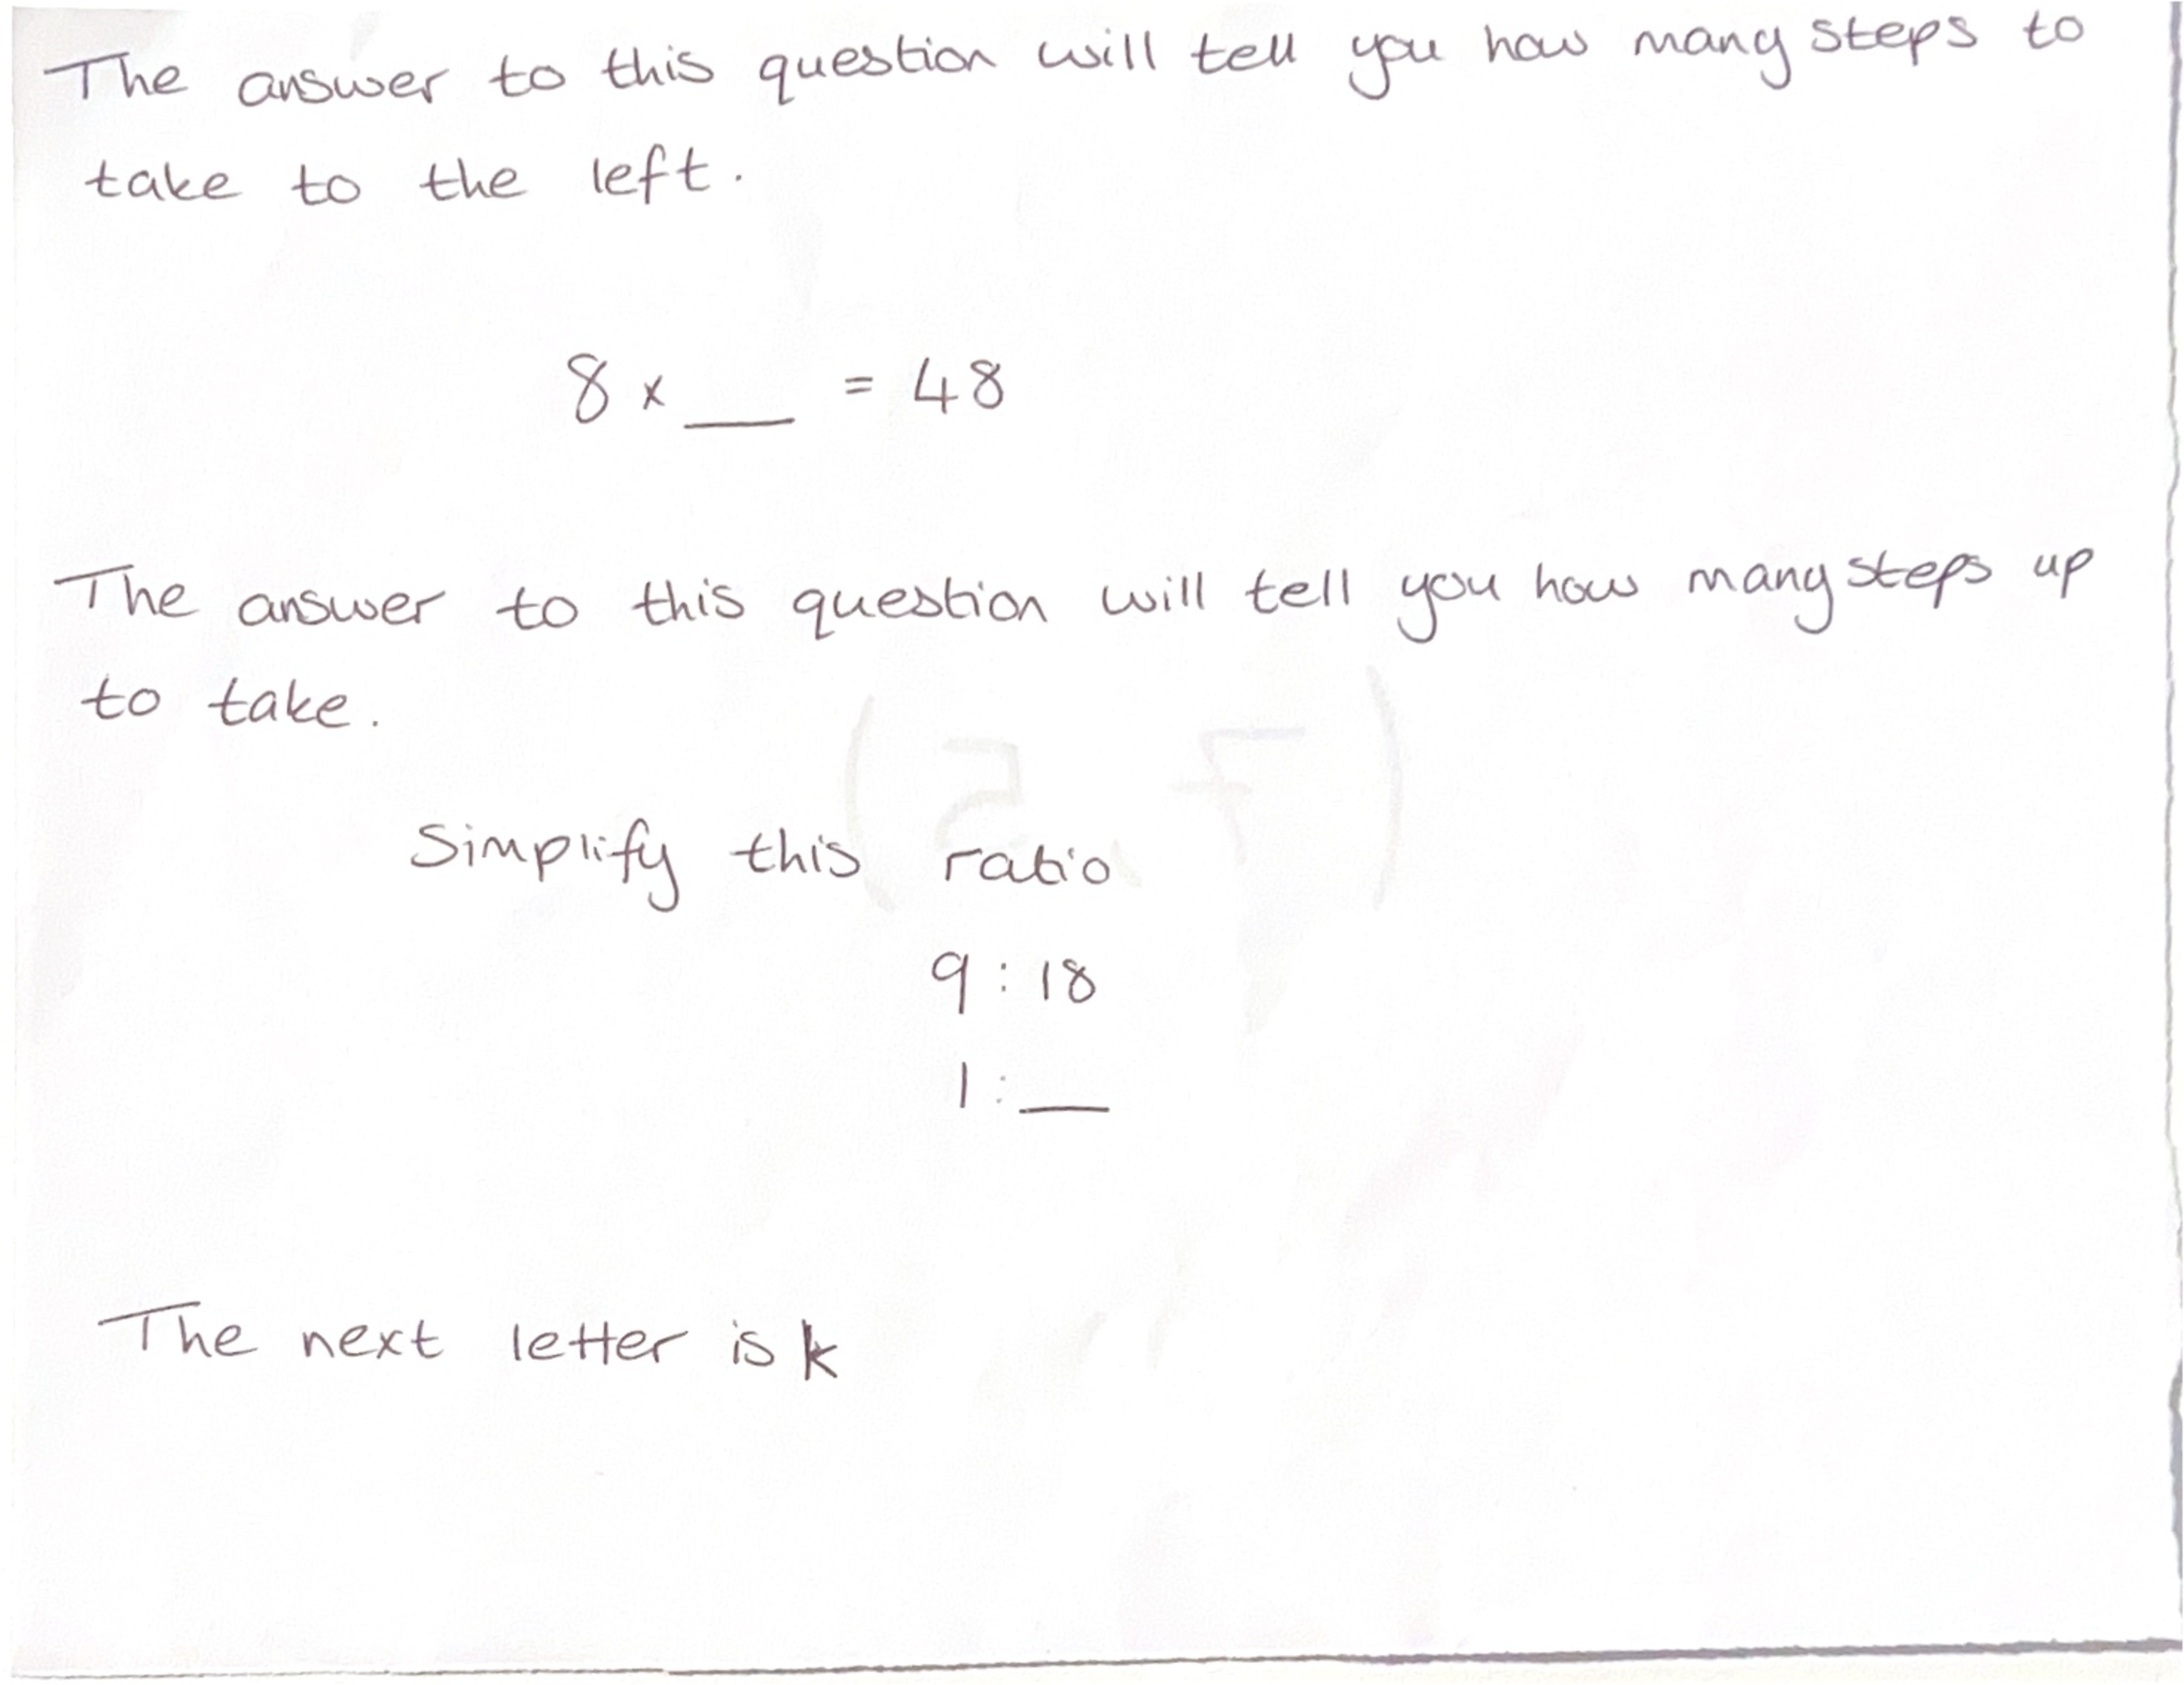
\includegraphics[width=\textwidth]{Images/CoordinateGrid_questions-pages-6.pdf}
\end{figure}

\end{document}